% =====================================================================
%  Laplace Transforms — A Self-Study Reference Deck
%  Beamer source file — compiles with pdflatex, xelatex, or tectonic
%
%  Style adapted from LaTeX_STYLE_GUIDE.md:
%    - Five-color palette (headerblue, accentgreen, accentorange, workpurple, warnred)
%    - Six box roles via tcolorbox (topicsbox, formulabox, methodbox,
%      examplebox, conceptbox, warningbox)
%    - Live solution tracking in workpurple
%    - Concept-takeaway emphasis in accentorange
%
%  Voice: academic formal, impersonal third-person.
%  No copyrighted material: no textbook citations, no direct quotes,
%  no source footers. Mathematical facts are public domain.
%
%  Compile:  pdflatex Laplace_Transforms_Deck.tex
%         or xelatex  Laplace_Transforms_Deck.tex
%         or tectonic Laplace_Transforms_Deck.tex
% =====================================================================

\documentclass[aspectratio=169,11pt]{beamer}

% ─── Engine detection ───
\usepackage{iftex}
\ifPDFTeX
  \usepackage[T1]{fontenc}
  \usepackage[utf8]{inputenc}
\else
  \usepackage{fontspec}
\fi

% ─── Core packages ───
\usepackage{amsmath,amssymb,amsthm}
\usepackage{mathtools}
\usepackage{xcolor}
\usepackage[most]{tcolorbox}
\usepackage{booktabs}
% Force math to wrap and prevent overflow
\allowdisplaybreaks
\usepackage{microtype} % Improves text justification and margin spacing
\setlength{\emergencystretch}{3em} % Allows LaTeX extra room to avoid overfull lines
\usepackage{array}
\usepackage{tabularx}
\usepackage{graphicx}
\usepackage{hyperref}
% bookmarks=false avoids writing \jobname.out, which tectonic cannot MD5
% when the filename contains spaces (quotes the jobname -> invalid path).
% (beamer loads hyperref itself, so set the option via \hypersetup, not \usepackage.)
\hypersetup{bookmarks=false}
\usepackage{tikz}
\usetikzlibrary{arrows,positioning,calc}

% Note: enumitem is incompatible with beamer in some configurations.
% Use beamer's native itemize/enumerate instead.

% ─── Palette (verbatim from LaTeX_STYLE_GUIDE.md) ───
\definecolor{headerblue}{HTML}{1C569E}
\definecolor{accentgreen}{HTML}{2E7D32}
\definecolor{accentorange}{HTML}{E27A1E}
\definecolor{workpurple}{HTML}{A020F0}
\definecolor{warnred}{HTML}{C0392B}

% ─── Beamer theme cleanup ───
\usetheme{default}
\setbeamertemplate{navigation symbols}{}
\setbeamersize{text margin left=10mm, text margin right=10mm}
\setbeamercolor{frametitle}{fg=headerblue}
\setbeamercolor{title}{fg=white}
\setbeamercolor{structure}{fg=headerblue}
\setbeamercolor{alerted text}{fg=accentorange}
\setbeamercolor{itemize item}{fg=headerblue}
\setbeamercolor{itemize subitem}{fg=accentorange}
\setbeamerfont{frametitle}{size=\large, series=\bfseries}
\setbeamerfont{title}{size=\Huge, series=\bfseries}

% Disable section/subsection pages to prevent recursion issues
\setbeamertemplate{section page}{}
\setbeamertemplate{subsection page}{}
% Do not insert section pages automatically
\setbeamertemplate{section in toc}[default]
\setbeamertemplate{subsection in toc}[default]

% Simple frametitle with accent rule underneath
\setbeamertemplate{frametitle}{%
  \vskip0.5ex
  \strut\insertframetitle\strut\par
  \vskip-0.2ex
  {\color{accentorange}\rule{\dimexpr\paperwidth-20mm\relax}{1pt}}%
  \vskip0.3ex
}

% Footer with page number
\setbeamertemplate{footline}{%
  \leavevmode%
  \hbox{%
    \begin{beamercolorbox}[wd=.5\paperwidth,ht=2.5ex,dp=1ex,leftskip=10mm]{}%
      {\tiny\color{gray}\insertshorttitle}%
    \end{beamercolorbox}%
    \begin{beamercolorbox}[wd=.5\paperwidth,ht=2.5ex,dp=1ex,rightskip=10mm]{}%
      \hfill{\tiny\color{gray}\insertframenumber\,/\,\inserttotalframenumber}%
    \end{beamercolorbox}%
  }%
}

% ─── Six box environments (from LaTeX_STYLE_GUIDE.md §3) ───
% 1. topicsbox — Blue Overview Capsule
\newtcolorbox{topicsbox}[1][Overview]{%
  enhanced, colback=headerblue!6!white, colframe=headerblue,
  coltitle=white, fonttitle=\bfseries\small,
  title=#1, boxrule=0.6pt, arc=2mm,
  left=3mm, right=3mm, top=1mm, bottom=1mm,
  fontupper=\footnotesize
}

% 2. formulabox — Orange Formula Container
\newtcolorbox{formulabox}[1][Formula]{%
  enhanced, colback=accentorange!8!white, colframe=accentorange,
  coltitle=white, fonttitle=\bfseries\small,
  title={#1}, boxrule=0.6pt, arc=1mm,
  left=3mm, right=3mm, top=1mm, bottom=1mm,
  fontupper=\footnotesize
}

% 3. methodbox — Green Algorithm Block
\newtcolorbox{methodbox}[1][Method]{%
  enhanced, colback=accentgreen!6!white, colframe=accentgreen,
  coltitle=white, fonttitle=\bfseries\small,
  title={#1}, boxrule=0.6pt, arc=1mm,
  left=3mm, right=3mm, top=1mm, bottom=1mm,
  fontupper=\footnotesize
}

% 4. examplebox — Purple West-Bordered Worked Example
\newtcolorbox{examplebox}[1][Worked Example]{%
  enhanced, colback=workpurple!4!white, colframe=workpurple,
  coltitle=white, fonttitle=\bfseries\small,
  title={#1}, boxrule=0.4pt, sharp corners,
  borderline west={3pt}{0pt}{workpurple},
  left=5mm, right=3mm, top=1mm, bottom=1mm,
  fontupper=\footnotesize
}

% 5. conceptbox — Orange Thin-Bordered Final Concept Takeaway
\newtcolorbox{conceptbox}[1][Key Takeaway]{%
  enhanced, colback=accentorange!5!white, colframe=accentorange,
  coltitle=white, fonttitle=\bfseries\small,
  title={#1}, boxrule=0.3pt, arc=1mm,
  left=3mm, right=3mm, top=1mm, bottom=1mm,
  fontupper=\footnotesize
}

% 6. warningbox — Crimson West-Bordered Common Pitfall
\newtcolorbox{warningbox}[1][Common Pitfall]{%
  enhanced, colback=red!3!white, colframe=warnred,
  coltitle=white, fonttitle=\bfseries\small,
  title={#1}, boxrule=0.4pt, sharp corners,
  borderline west={3pt}{0pt}{warnred},
  left=5mm, right=3mm, top=1mm, bottom=1mm,
  fontupper=\footnotesize
}

% ─── Inline color utilities (mirroring \textcolor{...}{...}) ───
\newcommand{\live}[1]{\textcolor{workpurple}{#1}}    % live solution tracking
\newcommand{\key}[1]{\textcolor{accentorange}{\textbf{#1}}}  % concept takeaway emphasis

% ─── Auto-shrink wide display math to text width ───
\newcommand{\resizeeq}[1]{\resizebox{\textwidth}{!}{$#1$}}

% ─── Title metadata ───
\title{Laplace Transforms}
\subtitle{A Self-Study Reference Deck}
\author{Personal Study Reference}
\date{}

% =====================================================================
\begin{document}
% =====================================================================

% ─── Slide 1: Cover ───
{
\setbeamercolor{background canvas}{bg=headerblue}
\setbeamertemplate{footline}{}
\begin{frame}[plain]
  \begin{tikzpicture}[overlay, remember picture]
    \fill[workpurple!30] (current page.south west) rectangle ([xshift=3cm]current page.north west);
  \end{tikzpicture}
  \vspace{2cm}
  \begin{center}
    {\color{accentorange}\small\textsc{A Self-Study Reference Deck}}\\[0.6cm]
    {\color{white}\Huge\textbf{Laplace Transforms}}\\[0.5cm]
    {\color{white!85}\large\itshape From the definition to the tautochrone ---\\
    a single-volume reference with worked examples,\\
    transform tables, and historical context.}\\[1cm]
    {\color{white!70}\footnotesize Personal study reference \quad\textbar\quad No external attribution}
  \end{center}
\end{frame}
}

% ─── Slide 2: Table of Contents ───
\begin{frame}{Contents --- Six Parts, Fifty-Five Slides}
\footnotesize
\begin{columns}[T]
\begin{column}{0.48\textwidth}
\begin{topicsbox}[Part I --- Foundations (9 slides)]
The definition, existence, uniqueness, linearity, and the power-series analogy.
\end{topicsbox}
\vspace{1mm}
\begin{topicsbox}[Part II --- The Transform Toolkit (10 slides)]
Shifting properties, Heaviside, Dirac delta, transforms of derivatives and integrals.
\end{topicsbox}
\vspace{1mm}
\begin{topicsbox}[Part III --- Solving ODEs (10 slides)]
The five-step method, worked examples, discontinuous and impulse forcing, linear systems.
\end{topicsbox}
\end{column}
\begin{column}{0.48\textwidth}
\begin{topicsbox}[Part IV --- Convolution \& Systems (8 slides)]
Convolution theorem, Duhamel's principle, Volterra equations, transfer functions, poles.
\end{topicsbox}
\vspace{1mm}
\begin{topicsbox}[Part V --- Advanced Applications (7 slides)]
PDEs via Laplace, beam bending, Abel's tautochrone, real-integral tricks, resonance.
\end{topicsbox}
\vspace{1mm}
\begin{topicsbox}[Part VI --- Reference \& Closing (9 slides)]
Master transform tables, encyclopedic worked examples, historical sketches, cheat-sheet.
\end{topicsbox}
\end{column}
\end{columns}
\end{frame}

% ═══════════════════════════════════════════════════════════════════
% PART I --- FOUNDATIONS
% ═══════════════════════════════════════════════════════════════════

\section{Part I --- Foundations}

% ─── Slide 3: Section Header Part I ───
{
\setbeamercolor{background canvas}{bg=headerblue}
\setbeamertemplate{footline}{}
\begin{frame}[plain]
\vspace{2cm}
{\color{accentorange}\Huge\textbf{PART I}}\\[0.4cm]
{\color{white}\Huge\textbf{Foundations}}\\[0.8cm]
{\color{white!85}\large Why Laplace? The two-domain picture. The definition.\\
Existence and uniqueness. Linearity. The power-series analogy.}
\end{frame}
}

% ─── Slide 4: Why Laplace? ───
\begin{frame}{Why Laplace? Two Domains and a Black Box}
\footnotesize
\begin{columns}[T]
\begin{column}{0.48\textwidth}
\begin{topicsbox}[The Pain Point]
Classical ODE methods --- undetermined coefficients, variation of parameters --- require continuity of the forcing function $f(t)$. Many physical inputs are discontinuous or impulsive: switch flips, hammer blows, voltage spikes, point loads. Stitching piecewise solutions by hand is tedious.
\end{topicsbox}
\vspace{0.5mm}
\begin{methodbox}[The Laplace Strategy]
Transform the IVP from the \emph{time domain} $t$ to the \emph{frequency domain} $s$. The derivative $d/dt$ becomes multiplication by $s$. Solve the resulting algebraic equation for $Y(s)$. Invert the transform to recover $y(t)$.
\end{methodbox}
\end{column}
\begin{column}{0.48\textwidth}
\centering
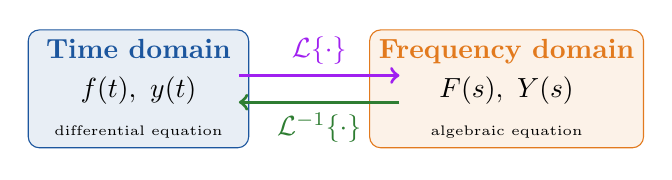
\begin{tikzpicture}[scale=0.85]
\node[draw=headerblue, fill=headerblue!10, rounded corners, minimum width=2.8cm, minimum height=1.4cm, align=center] at (0,2) {\textbf{\color{headerblue}Time domain}\\[2pt]$f(t),\ y(t)$\\[2pt]\tiny differential equation};
\node[draw=accentorange, fill=accentorange!10, rounded corners, minimum width=2.8cm, minimum height=1.4cm, align=center] at (5.5,2) {\textbf{\color{accentorange}Frequency domain}\\[2pt]$F(s),\ Y(s)$\\[2pt]\tiny algebraic equation};
\draw[->, workpurple, very thick] (1.5,2.2) -- (3.9,2.2) node[midway, above, workpurple] {$\mathcal{L}\{\cdot\}$};
\draw[->, accentgreen, very thick] (3.9,1.8) -- (1.5,1.8) node[midway, below, accentgreen] {$\mathcal{L}^{-1}\{\cdot\}$};
\end{tikzpicture}
\end{column}
\end{columns}
\end{frame}

% ─── Slide 4 (cont.): Why Laplace takeaway ───
\begin{frame}{Why Laplace? Two Domains and a Black Box (cont.)}
\footnotesize
\begin{conceptbox}[The Takeaway]
A differential equation becomes an algebraic equation --- initial conditions are absorbed automatically, and discontinuous forcing is handled natively.
\end{conceptbox}
\end{frame}

% ─── Slide 5: Definition and Notation ───
\begin{frame}{The Laplace Transform --- Definition and Notation}
\footnotesize
\begin{formulabox}[Master Formula]
\[
\mathcal{L}\{f(t)\} \;=\; F(s) \;=\; \int_0^{\infty} e^{-st}\, f(t)\, dt
\]
\end{formulabox}
\vspace{0.5mm}
\begin{columns}[T]
\begin{column}{0.48\textwidth}
\begin{topicsbox}[Notation Conventions]
\begin{itemize}
\item Lowercase $f, g, y$ for time-domain functions
\item Uppercase $F, G, Y$ for their Laplace transforms
\item $s$ is generally complex: $s = \sigma + i\omega$
\item Lower limit $0^{-}$ captures impulses $\delta(t)$ at the origin
\end{itemize}
\end{topicsbox}
\end{column}
\begin{column}{0.48\textwidth}
\begin{warningbox}[The $0^{-}$ Subtlety]
When the integrand includes $\delta(t)$, the lower limit must be $0^{-}$ so the impulse is captured. Without it, $\mathcal{L}\{\delta(t)\} = 1$ would fail.
\end{warningbox}
\end{column}
\end{columns}
\vspace{0.5mm}
\begin{methodbox}[Domain of $s$]
The integral converges absolutely for $s$ large enough: $\mathrm{Re}(s) > \alpha$, where $\alpha$ is the exponential-order bound on $f$.
\end{methodbox}
\end{frame}

% ─── Slide 6: Starter Transforms ───
\begin{frame}{The Starter Transforms}
\footnotesize
\begin{topicsbox}[Six Transform Pairs to Know]
\centering
\begin{tabular}{@{}lll@{}}
\toprule
\textbf{$f(t)$} & \textbf{$F(s) = \mathcal{L}\{f(t)\}$} & \textbf{Valid for} \\
\midrule
$1$ & $\dfrac{1}{s}$ & $s > 0$ \\
$t$ & $\dfrac{1}{s^2}$ & $s > 0$ \\
$t^n,\ n\in\mathbb{N}$ & $\dfrac{n!}{s^{n+1}}$ & $s > 0$ \\
$e^{at}$ & $\dfrac{1}{s-a}$ & $s > a$ \\
$\sin(at)$ & $\dfrac{a}{s^2+a^2}$ & $s > 0$ \\
$\cos(at)$ & $\dfrac{s}{s^2+a^2}$ & $s > 0$ \\
\bottomrule
\end{tabular}
\end{topicsbox}
\end{frame}

% ─── Slide 6 (cont.): starter derivations ───
\begin{frame}{The Starter Transforms (cont.)}
\footnotesize
\begin{columns}[T]
\begin{column}{0.48\textwidth}
\begin{examplebox}[Deriving $\mathcal{L}\{1\}$]
\[\mathcal{L}\{1\} = \int_0^{\infty} e^{-st}\,dt = \left[-\frac{1}{s}e^{-st}\right]_0^{\infty} = \frac{1}{s}\]
For $s > 0$, the boundary term at $\infty$ vanishes.
\end{examplebox}
\end{column}
\begin{column}{0.48\textwidth}
\begin{examplebox}[Deriving $\mathcal{L}\{e^{at}\}$]
\[\mathcal{L}\{e^{at}\} = \int_0^{\infty} e^{-(s-a)t}\,dt = \frac{1}{s-a}\]
For $s > a$. Same pattern as $\mathcal{L}\{1\}$ with $s \to s-a$.
\end{examplebox}
\end{column}
\end{columns}
\end{frame}

% ─── Slide 7: The Euler Trick ───
\begin{frame}{The Euler Trick --- $\sin$ and $\cos$ from $e^{ibt}$}
\footnotesize
\begin{examplebox}[Worked Example]
\textbf{Step 1.} From the table, $\mathcal{L}\{e^{at}\} = \frac{1}{s-a}$ for $s > a$. Substitute $a = ib$ (where $b$ is real):
\[\mathcal{L}\{e^{ibt}\} = \frac{1}{s - ib}\]

\textbf{Step 2.} Multiply numerator and denominator by the conjugate $s + ib$:
\[\mathcal{L}\{e^{ibt}\} = \frac{s + ib}{s^2 + b^2}\]

\textbf{Step 3.} Apply Euler's formula $e^{ibt} = \cos(bt) + i\sin(bt)$ and use linearity:
\[\mathcal{L}\{\cos(bt) + i\sin(bt)\} = \frac{s}{s^2+b^2} + i\,\frac{b}{s^2+b^2}\]

\textbf{Step 4.} Equate real and imaginary parts:
\[\mathcal{L}\{\cos(bt)\} = \frac{s}{s^2+b^2}, \qquad \mathcal{L}\{\sin(bt)\} = \frac{b}{s^2+b^2}\]
\end{examplebox}
\end{frame}

% ─── Slide 7 (cont.): Euler Trick takeaway ───
\begin{frame}{The Euler Trick --- $\sin$ and $\cos$ from $e^{ibt}$ (cont.)}
\footnotesize
\begin{conceptbox}[Key Takeaway]
Complex $s$ is not a complication --- it is a unification. Sines and cosines are projections of complex exponentials, so their transforms follow immediately from $\mathcal{L}\{e^{at}\}$.
\end{conceptbox}
\end{frame}

% ─── Slide 8: Existence Theorem ───
\begin{frame}{When Does $\mathcal{L}\{f\}$ Exist?}
\footnotesize
\begin{columns}[T]
\begin{column}{0.42\textwidth}
\begin{formulabox}[Two Sufficient Conditions]
\textbf{(a)} $f$ is \emph{piecewise continuous} on every finite $[0,b]$: finitely many jumps, one-sided limits exist.

\medskip
\textbf{(b)} $f$ is of \emph{exponential order}: $\exists\, M, \alpha, t_0$ such that $|f(t)| \le M e^{\alpha t}$ for $t > t_0$.
\end{formulabox}
\vspace{0.5mm}
\begin{conceptbox}[Existence Theorem]
If $f$ is piecewise continuous on every $[0,b]$ and of exponential order $e^{\alpha t}$, then $\mathcal{L}\{f\}$ exists for $s > \alpha$.
\end{conceptbox}
\end{column}
\begin{column}{0.56\textwidth}
\begin{methodbox}[Proof Sketch (Comparison Test)]
\textbf{Step 1.} Split: $\int_0^{\infty} = \int_0^{t_0} + \int_{t_0}^{\infty}$. The first piece exists by piecewise continuity.

\textbf{Step 2.} For the tail, use exponential order:
\[|e^{-st}f(t)| \le M e^{-(s-\alpha)t}\]

\textbf{Step 3.} The dominating integral converges for $s > \alpha$:
\[\int_{t_0}^{\infty} M e^{-(s-\alpha)t}\,dt = \frac{M}{s-\alpha}\,e^{-(s-\alpha)t_0}\]

\textbf{Step 4.} Apply the comparison test $\Rightarrow$ $\mathcal{L}\{f\}$ converges absolutely.
\end{methodbox}
\vspace{0.5mm}
\begin{warningbox}[Sufficient, not necessary]
$f(t) = t^{-1/2}$ is not piecewise continuous at $t=0$, yet $\mathcal{L}\{t^{-1/2}\} = \sqrt{\pi/s}$ exists via $t = u^2$.
\end{warningbox}
\end{column}
\end{columns}
\end{frame}

% ─── Slide 9: Uniqueness Theorem ───
\begin{frame}{When Is $\mathcal{L}^{-1}\{F\}$ Unique?}
\footnotesize
\begin{columns}[T]
\begin{column}{0.48\textwidth}
\begin{formulabox}[Uniqueness Theorem]
If $f$ and $g$ are \emph{continuous} on $[0,\infty)$ and of exponential order, and $\mathcal{L}\{f\} = \mathcal{L}\{g\}$ for all $s > C$, then $f(t) = g(t)$ for all $t \ge 0$.
\end{formulabox}
\vspace{0.5mm}
\begin{conceptbox}[Why we require continuity]
The Laplace integral cannot distinguish functions that differ only at finitely many points. Uniqueness holds only for \emph{continuous} inverses --- which is fine, since solutions of ODEs are continuous.
\end{conceptbox}
\end{column}
\begin{column}{0.48\textwidth}
\begin{examplebox}[Counterexample]
Define
\[g(t) = \begin{cases} 1, & 0 < t < 3 \\ 2, & t = 3 \\ 1, & t > 3 \end{cases}\]
Then $\mathcal{L}\{g\} = \frac{1}{s}$ for $s > 0$, which equals $\mathcal{L}\{1\}$. But clearly $g(t) \ne 1$ at $t=3$.

\medskip
The \emph{continuous} inverse of $1/s$ is $f(t) = 1$.
\end{examplebox}
\vspace{0.5mm}
\begin{warningbox}[Heaviside at zero]
$u(0) = 0$, $u(0) = \tfrac{1}{2}$, and $u(0) = 1$ all give the same transform $1/s$. The value at the discontinuity is invisible.
\end{warningbox}
\end{column}
\end{columns}
\end{frame}

% ─── Slide 10: Power-Series Analogy ───
\begin{frame}{Laplace Transforms as Continuous Power Series}
\footnotesize
\begin{columns}[T]
\begin{column}{0.42\textwidth}
\begin{topicsbox}[The Analogy]
A power series: $\displaystyle\sum_{n=0}^{\infty} a(n)\, x^n$.

Its natural continuous analog: $\displaystyle\int_0^{\infty} a(t)\, x^t\, dt$.

Substitute $x = e^{-p}$:
\[\int_0^{\infty} a(t)\, e^{-pt}\, dt = \mathcal{L}\{a(t)\}\]

\medskip
The analogy suggests that Laplace transforms occupy in continuous analysis a role parallel to that of power series in discrete analysis.
\end{topicsbox}
\end{column}
\begin{column}{0.56\textwidth}
\begin{methodbox}[Why the Analogy Matters]
\begin{enumerate}
\item \textbf{Convergence theory.} Power series converge inside a radius; Laplace transforms converge in a half-plane $\mathrm{Re}(s) > \alpha$. The half-plane is the continuous analog of the radius.
\item \textbf{Operations.} Term-by-term differentiation of a power series corresponds to differentiation under the integral sign of a Laplace transform.
\item \textbf{Inversion.} A power series is recovered from its coefficients; a Laplace transform is recovered via the Bromwich inversion integral.
\end{enumerate}
\end{methodbox}
\vspace{0.5mm}
\begin{conceptbox}[Key Takeaway]
The Laplace transform is the natural continuous counterpart of the power series --- the most useful discrete representation in analysis.
\end{conceptbox}
\end{column}
\end{columns}
\end{frame}

% ─── Slide 11: Linearity ───
\begin{frame}{Linearity and the Product Warning}
\footnotesize
\begin{columns}[T]
\begin{column}{0.48\textwidth}
\begin{formulabox}[Linearity Theorem]
If $\mathcal{L}\{f\}$ and $\mathcal{L}\{g\}$ exist, then for any constants $\alpha, \beta$:
\[\mathcal{L}\{\alpha f + \beta g\} = \alpha\,\mathcal{L}\{f\} + \beta\,\mathcal{L}\{g\}\]
The inverse $\mathcal{L}^{-1}$ inherits linearity.
\end{formulabox}
\vspace{0.5mm}
\begin{examplebox}[Combining Transforms]
\[\mathcal{L}\{2 + 5t + 9e^{-2t}\} = \frac{2}{s} + \frac{5}{s^2} + \frac{9}{s+2}\]
No integration required --- pure table lookup plus linearity.
\end{examplebox}
\end{column}
\begin{column}{0.48\textwidth}
\begin{warningbox}[CRITICAL: $\mathcal{L}\{f \cdot g\} \ne \mathcal{L}\{f\} \cdot \mathcal{L}\{g\}$]
A product in the time domain does \emph{not} transform into a product in the frequency domain. The correct product rule is the \emph{convolution theorem}: $\mathcal{L}\{f * g\} = \mathcal{L}\{f\}\cdot\mathcal{L}\{g\}$, where $*$ denotes convolution.
\end{warningbox}
\vspace{0.5mm}
\begin{examplebox}[Why the Warning Matters]
\emph{Wrong:} $\mathcal{L}\{t\sin t\} \ne \frac{1}{s^2}\cdot\frac{1}{s^2+1}$.

\emph{Right} (use $\mathcal{L}\{t f(t)\} = -F'(s)$):
\[\mathcal{L}\{t\sin t\} = -\frac{d}{ds}\!\left[\frac{1}{s^2+1}\right] = \frac{2s}{(s^2+1)^2}\]
\end{examplebox}
\end{column}
\end{columns}
\end{frame}

% ─── Slide 11 (cont.): Linearity takeaway ───
\begin{frame}{Linearity and the Product Warning (cont.)}
\footnotesize
\begin{conceptbox}[Key Takeaway]
Linearity is a friend; naive multiplication is an enemy. The transform converts sums into sums --- but converts \emph{convolutions} into products.
\end{conceptbox}
\end{frame}

% ═══════════════════════════════════════════════════════════════════
% PART II --- THE TRANSFORM TOOLKIT
% ═══════════════════════════════════════════════════════════════════

\section{Part II --- The Transform Toolkit}

% ─── Slide 12: Section Header Part II ───
{
\setbeamercolor{background canvas}{bg=headerblue}
\setbeamertemplate{footline}{}
\begin{frame}[plain]
\vspace{2cm}
{\color{accentorange}\Huge\textbf{PART II}}\\[0.4cm]
{\color{white}\Huge\textbf{The Transform Toolkit}}\\[0.8cm]
{\color{white!85}\large Shifting properties. The Heaviside function. The Dirac delta.\\
Transforms of derivatives and integrals. The full operational calculus.}
\end{frame}
}

% ─── Slide 13: First Shifting Property ───
\begin{frame}{First Shifting Property (Translation in $s$)}
\footnotesize
\begin{columns}[T]
\begin{column}{0.42\textwidth}
\begin{formulabox}[The Rule]
\[\mathcal{L}\{e^{at} f(t)\} = F(s - a)\]
where $F(s) = \mathcal{L}\{f(t)\}$. Inversely, $\mathcal{L}^{-1}\{F(s-a)\} = e^{at} f(t)$.
\end{formulabox}
\vspace{0.5mm}
\begin{methodbox}[How to Use It]
A denominator like $(s-a)^2 + b^2$ is recognized as $s^2 + b^2$ shifted by $a$. The inverse is $e^{at}\sin(bt)$. Same trick for $(s-a)^{n+1} \to e^{at} t^n / n!$.
\end{methodbox}
\end{column}
\begin{column}{0.56\textwidth}
\begin{examplebox}[$\mathcal{L}\{e^{at}\sin(bt)\}$]
From the table, $\mathcal{L}\{\sin(bt)\} = \frac{b}{s^2 + b^2}$. By the first shifting property:
\[\mathcal{L}\{e^{at}\sin(bt)\} = \frac{b}{(s-a)^2 + b^2}, \quad s > a\]
\end{examplebox}
\vspace{0.5mm}
\begin{examplebox}[$\mathcal{L}^{-1}\!\left\{\frac{1}{s^2+4s+8}\right\}$]
Complete the square: $s^2+4s+8 = (s+2)^2 + 4$. So
\[\frac{1}{s^2+4s+8} = \frac{1}{(s+2)^2 + 2^2}\]
Recognize $\frac{b}{(s-a)^2+b^2}$ with $b=2, a=-2$, missing a factor of $2$:
\[\mathcal{L}^{-1}\!\left\{\frac{1}{(s+2)^2+4}\right\} = \frac{1}{2}\,e^{-2t}\sin(2t)\]
\end{examplebox}
\end{column}
\end{columns}
\end{frame}

% ─── Slide 13 (cont.): First Shifting takeaway ───
\begin{frame}{First Shifting Property (Translation in $s$) (cont.)}
\footnotesize
\begin{conceptbox}[Key Takeaway]
Whenever a denominator has the form $(s-a)^2 + b^2$ or $(s-a)^{n+1}$, the first shifting property gives the inverse immediately --- no partial fractions needed.
\end{conceptbox}
\end{frame}

% ─── Slide 14: Second Shifting Property ───
\begin{frame}{Second Shifting Property (Translation in $t$)}
\footnotesize
\begin{columns}[T]
\begin{column}{0.42\textwidth}
\begin{formulabox}[The Rule]
\[\mathcal{L}\{u_a(t)\, f(t-a)\} = e^{-as}\, F(s)\]
where $u_a(t) = u(t-a)$ is the Heaviside step at $t = a$, and $F(s) = \mathcal{L}\{f(t)\}$.

\medskip
Inversely: $\mathcal{L}^{-1}\{e^{-as} F(s)\} = u_a(t)\, f(t-a)$.
\end{formulabox}
\vspace{0.5mm}
\begin{methodbox}[How to Use It]
If $e^{-as}$ multiplies a recognizable transform, the inverse is the un-shifted inverse \emph{delayed by $a$} and \emph{zeroed before $t = a$}.
\end{methodbox}
\end{column}
\begin{column}{0.56\textwidth}
\begin{examplebox}[$\mathcal{L}\{u_a(t)\}$]
Take $f(t) = 1$. Then $F(s) = 1/s$, so:
\[\mathcal{L}\{u_a(t)\} = \frac{e^{-as}}{s}, \quad s > 0\]
\end{examplebox}
\vspace{0.5mm}
\begin{examplebox}[$\mathcal{L}^{-1}\!\left\{e^{-4s}\!\left(\frac{2}{s^2}+\frac{5}{s}\right)\right\}$]
Recognize $F(s) = 2/s^2 + 5/s$. Its inverse is $f(t) = 2t + 5$. Apply the second shifting property with $a = 4$:
\resizeeq{\mathcal{L}^{-1}\{e^{-4s} F(s)\} = u_4(t)\, f(t-4) = u_4(t)\,[2(t-4)+5] = u_4(t)\,(2t-3)}
This is $0$ for $t < 4$ and $2t - 3$ for $t > 4$.
\end{examplebox}
\end{column}
\end{columns}
\end{frame}

% ─── Slide 14 (cont.): Second Shifting takeaway ───
\begin{frame}{Second Shifting Property (Translation in $t$) (cont.)}
\footnotesize
\begin{conceptbox}[Key Takeaway]
$e^{-as}$ in the $s$-domain is a \emph{time delay} $a$ in the $t$-domain. This is the foundation for switched circuits, delayed forcing, and piecewise inputs.
\end{conceptbox}
\end{frame}

% ─── Slide 15: The Heaviside Function ───
\begin{frame}{The Unit Step Function as a Building Block}
\footnotesize
\begin{columns}[T]
\begin{column}{0.58\textwidth}
\begin{formulabox}[Definition]
\[u_a(t) = u(t-a) = \begin{cases} 0, & t < a \\ 1, & t \ge a \end{cases}\]
A jump discontinuity of size $+1$ at $t = a$. The value at the discontinuity is invisible to $\mathcal{L}$.
\end{formulabox}
\vspace{0.5mm}
\begin{methodbox}[Three Uses]
\textbf{(a) Switched inputs:} $V_0\, u_a(t)$ is a constant voltage switched on at $t = a$.

\textbf{(b) Box functions:} $M[u_a(t) - u_b(t)]$ is $M$ on $[a,b]$ and $0$ elsewhere.

\textbf{(c) Piecewise functions:} any piecewise $f$ is $\sum_k u_{a_k}(t)\, f_k(t - a_k)$.
\end{methodbox}
\end{column}
\begin{column}{0.38\textwidth}
\centering
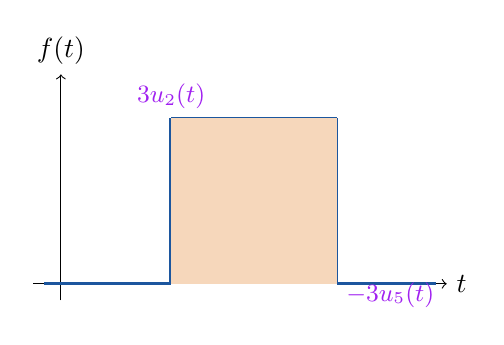
\begin{tikzpicture}[scale=0.7]
\draw[->] (-0.5,0) -- (7,0) node[right] {$t$};
\draw[->] (0,-0.3) -- (0,3.8) node[above] {$f(t)$};
\draw[headerblue, very thick] (-0.3,0) -- (2,0);
\draw[headerblue, very thick] (2,0) -- (2,3);
\draw[headerblue, very thick] (2,3) -- (5,3);
\draw[headerblue, very thick] (5,3) -- (5,0);
\draw[headerblue, very thick] (5,0) -- (6.8,0);
\fill[accentorange!30] (2,0) rectangle (5,3);
\node[workpurple, above] at (2,3) {\small $3u_2(t)$};
\node[workpurple, below right] at (5,0.2) {\small $-3u_5(t)$};
\end{tikzpicture}
\end{column}
\end{columns}
\end{frame}

% ─── Slide 15 (cont.): box function example ───
\begin{frame}{The Unit Step Function as a Building Block (cont.)}
\footnotesize
\begin{examplebox}[A Box Function]
$f(t) = 3$ on $[2,5]$ and $0$ elsewhere: $f(t) = 3u_2(t) - 3u_5(t)$.
\[\mathcal{L}\{f\} = \frac{3(e^{-2s} - e^{-5s})}{s}\]
\end{examplebox}
\end{frame}

% ─── Slide 16: Piecewise via Heaviside ───
\begin{frame}{Encoding Piecewise Functions with Heaviside}
\footnotesize
\begin{columns}[T]
\begin{column}{0.32\textwidth}
\begin{examplebox}[Single Step]
$f(t) = 5$ for $t<2$, $0$ for $t>2$.

Express as $5(1 - u_2(t))$:
\[\mathcal{L}\{f\} = \frac{5(1-e^{-2s})}{s}\]
\end{examplebox}
\end{column}
\begin{column}{0.32\textwidth}
\begin{examplebox}[Box Pulse]
$f(t) = 0$ for $t<2$, $3$ for $2<t<5$, $0$ for $t>5$.

Express as $3u_2(t) - 3u_5(t)$:
\[\mathcal{L}\{f\} = \frac{3(e^{-2s}-e^{-5s})}{s}\]
\end{examplebox}
\end{column}
\begin{column}{0.32\textwidth}
\begin{examplebox}[Triangular Pulse]
$f(t) = t$ on $[0,1]$, $-t+2$ on $[1,2]$, $0$ elsewhere.

Write $f(t) = t - 2(t-1)u_1(t) + (t-2)u_2(t)$:
\[\mathcal{L}\{f\} = \frac{1 - 2e^{-s} + e^{-2s}}{s^2}\]
\end{examplebox}
\end{column}
\end{columns}
\vspace{1mm}
\begin{conceptbox}[Pattern]
Each piecewise function is a linear combination of $u_a(t)$ terms. The second shifting property then gives each term's transform as $e^{-as}$ times the transform of the shifted function.
\end{conceptbox}
\end{frame}

% ─── Slide 17: The Dirac Delta Function ───
\begin{frame}{The Dirac Delta Function}
\footnotesize
\begin{columns}[T]
\begin{column}{0.58\textwidth}
\begin{formulabox}[Definition (as a Limit)]
\[\delta(t - t_0) = \lim_{\alpha \to 0} \frac{1}{2\alpha}\,[u_{t_0-\alpha}(t) - u_{t_0+\alpha}(t)]\]
A rectangular pulse of width $2\alpha$ and height $1/(2\alpha)$ --- area is always $1$.
\end{formulabox}
\vspace{0.5mm}
\begin{formulabox}[Defining Properties]
\[\delta(t - t_0) = 0 \text{ for } t \ne t_0, \qquad \int_{-\infty}^{\infty} \delta(t-t_0)\,dt = 1\]
Informally: $\delta(0) = \infty$, zero elsewhere, total integral $1$. Strictly: $\delta$ is a \emph{generalized function} (distribution).
\end{formulabox}
\end{column}
\begin{column}{0.38\textwidth}
\centering
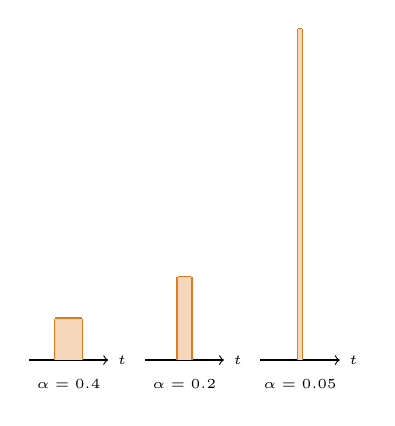
\begin{tikzpicture}[scale=0.42]
\foreach \a/\xoff in {0.4/0, 0.2/3.5, 0.05/7} {
  \begin{scope}[xshift=\xoff cm]
    \draw[->] (-1.2,0) -- (1.2,0) node[right] {\tiny $t$};
    \draw[accentorange, very thick] (-\a,0) -- (-\a, {1/(2*\a)});
    \draw[accentorange, very thick] (-\a, {1/(2*\a)}) -- (\a, {1/(2*\a)});
    \draw[accentorange, very thick] (\a, {1/(2*\a)}) -- (\a, 0);
    \fill[accentorange!30] (-\a,0) rectangle (\a, {1/(2*\a)});
    \node[below] at (0,-0.3) {\tiny $\alpha=\a$};
  \end{scope}
}
\end{tikzpicture}\\[2mm]
{\footnotesize\color{workpurple}$\delta(t) = \lim_{\alpha\to 0}$ of unit-area pulses}
\vspace{1mm}
\begin{conceptbox}[Physical Interpretation]
$\delta(t-t_0)$ models an idealized impulse: hammer blow, lightning strike, voltage spike, point load.
\end{conceptbox}
\end{column}
\end{columns}
\end{frame}

% ─── Slide 17 (cont.): Dirac --- rigor note ───
\begin{frame}{The Dirac Delta Function (cont.)}
\footnotesize
\begin{warningbox}[Common Pitfall]
$\delta(t)$ is \emph{not} a function in the classical sense. The rigorous foundation is the theory of distributions (Schwartz, 1940s).
\end{warningbox}
\end{frame}

% ─── Slide 18: Sifting Property ───
\begin{frame}{The Sifting Property and $\mathcal{L}\{\delta\}$}
\footnotesize
\begin{columns}[T]
\begin{column}{0.42\textwidth}
\begin{formulabox}[Sifting Property]
For any bounded continuous $g$:
\[\int_{-\infty}^{\infty} \delta(t-t_0)\, g(t)\, dt = g(t_0)\]
The delta function ``sifts out'' the value of $g$ at $t_0$.
\end{formulabox}
\vspace{0.5mm}
\begin{conceptbox}[$\delta$ is the Identity for Convolution]
\[(f * \delta)(t) = \int_0^t f(\tau)\,\delta(t-\tau)\,d\tau = f(t)\]
So $\delta$ is the multiplicative identity for convolution, even though $1$ is \emph{not} (recall $f * 1 \ne f$).
\end{conceptbox}
\end{column}
\begin{column}{0.56\textwidth}
\begin{methodbox}[Deriving $\mathcal{L}\{\delta(t-t_0)\}$]
Apply the sifting property with $g(t) = e^{-st}$:
\[\mathcal{L}\{\delta(t-t_0)\} = \int_{0^{-}}^{\infty} e^{-st}\,\delta(t-t_0)\,dt = e^{-st_0}\]
Special case $t_0 = 0$: $\mathcal{L}\{\delta(t)\} = 1$.
\end{methodbox}
\vspace{0.5mm}
\begin{examplebox}[Impulse Forcing]
Solve $y'' + 2y' + 26y = \delta_4(t)$, $y(0)=1, y'(0)=0$ (damped oscillator struck at $t=4$).

Transform: $s^2Y - s + 2(sY-2) + 26Y = e^{-4s}$. Solve:
\[Y(s) = \frac{s+2}{s^2+2s+26} + \frac{e^{-4s}}{s^2+2s+26}\]
Invert (using $(s+1)^2 + 25$):
\resizeeq{y(t) = e^{-t}\cos(5t) + \tfrac{1}{5}e^{-t}\sin(5t) + u_4(t)\cdot\tfrac{1}{5}e^{-(t-4)}\sin(5(t-4))}
\end{examplebox}
\end{column}
\end{columns}
\end{frame}

% ─── Slide 19: Transforms of Derivatives ───
\begin{frame}{Transforms of Derivatives --- The ODE Engine}
\footnotesize
\begin{columns}[T]
\begin{column}{0.42\textwidth}
\begin{formulabox}[The Three Rules]
\resizeeq{\begin{aligned}
\mathcal{L}\{f'(t)\} &= sF(s) - f(0) \\
\mathcal{L}\{f''(t)\} &= s^2 F(s) - s f(0) - f'(0) \\
\mathcal{L}\{f^{(n)}(t)\} &= s^n F(s) - s^{n-1}f(0) - \cdots - f^{(n-1)}(0)
\end{aligned}}
\end{formulabox}
\vspace{0.5mm}
\begin{methodbox}[Proof Sketch (Integration by Parts)]
\resizeeq{\begin{aligned}
\mathcal{L}\{f'\} &= \int_0^{\infty} e^{-st} f'(t)\,dt \\
&= \big[e^{-st}f(t)\big]_0^{\infty} + s\!\int_0^{\infty}\! e^{-st}f(t)\,dt \\
&= -f(0) + sF(s)
\end{aligned}}
The boundary term at $\infty$ vanishes by exponential order.
\end{methodbox}
\end{column}
\begin{column}{0.56\textwidth}
\begin{examplebox}[Worked Example --- Why This Matters]
Solve $y'' + 7y' + 10y = 0$, $y(0)=1, y'(0)=1$.

\textbf{Step 1.} Transform:
\[[s^2Y - s - 1] + 7[sY - 1] + 10Y = 0\]

\textbf{Step 2.} Solve algebraically:
\resizeeq{Y(s) = \frac{s+8}{s^2+7s+10} = \frac{2}{s+2} - \frac{1}{s+5}}

\textbf{Step 3.} Invert: $y(t) = 2e^{-2t} - e^{-5t}$.

\medskip
The initial conditions are baked in --- no separate solve for $c_1, c_2$.
\end{examplebox}
\vspace{0.5mm}
\begin{conceptbox}[Key Takeaway]
Differentiation in $t$ becomes multiplication by $s$. A linear ODE with constant coefficients becomes a purely algebraic equation for $Y(s)$.
\end{conceptbox}
\end{column}
\end{columns}
\end{frame}

% ─── Slide 19 (cont.): derivatives --- 0^- convention ───
\begin{frame}{Transforms of Derivatives --- The ODE Engine (cont.)}
\footnotesize
\begin{warningbox}[The $0^{-}$ Convention]
When impulses $\delta(t)$ are present, write $f(0^{-})$ instead of $f(0)$ --- the \emph{pre-initial condition}.
\end{warningbox}
\end{frame}

% ─── Slide 20: Transforms of Integrals ───
\begin{frame}{Transforms of Integrals --- and Integral Equations}
\footnotesize
\begin{columns}[T]
\begin{column}{0.42\textwidth}
\begin{formulabox}[The Integral Rule]
\[\mathcal{L}\!\left\{\int_0^t f(\tau)\,d\tau\right\} = \frac{F(s)}{s}\]
\textbf{Proof.} Let $g(t) = \int_0^t f(\tau)\,d\tau$. Then $g'(t) = f(t)$ and $g(0) = 0$. Apply the derivative rule: $\mathcal{L}\{g'\} = sG(s) - g(0) = sG(s)$. But $\mathcal{L}\{g'\} = F(s)$. So $G(s) = F(s)/s$.
\end{formulabox}
\vspace{0.5mm}
\begin{methodbox}[Inverting $F(s)/s$]
\[\mathcal{L}^{-1}\!\left\{\frac{F(s)}{s}\right\} = \int_0^t f(\tau)\,d\tau\]
A $1/s$ factor represents a time-domain integration.
\end{methodbox}
\end{column}
\begin{column}{0.56\textwidth}
\begin{examplebox}[A Volterra Integral Equation]
Solve $x(t) - t = \int_0^t x(\tau)\,d\tau$.

Transform both sides (using the integral rule on the RHS):
\[X(s) - \frac{1}{s^2} = \frac{X(s)}{s}\]
Solve algebraically:
\resizeeq{X(s)\!\left(1 - \frac{1}{s}\right) = \frac{1}{s^2} \;\Rightarrow\; X(s) = \frac{1}{s(s-1)} = \frac{1}{s-1} - \frac{1}{s}}
Invert: $x(t) = e^t - 1$.

\medskip
A differential equation and an integral equation become the same algebraic equation in the $s$-domain.
\end{examplebox}
\vspace{0.5mm}
\begin{conceptbox}[Key Takeaway]
Integration in $t$ becomes division by $s$. Integral equations become algebraic equations just as cleanly as differential equations.
\end{conceptbox}
\end{column}
\end{columns}
\end{frame}

% ─── Slide 21: Differentiation & Integration of Transforms ───
\begin{frame}{Differentiation and Integration of Transforms}
\footnotesize
\begin{columns}[T]
\begin{column}{0.48\textwidth}
\begin{formulabox}[Two More Rules]
\textbf{Differentiation in $s$:}
\[\mathcal{L}\{t\,f(t)\} = -F'(s)\]
\[\mathcal{L}\{t^n f(t)\} = (-1)^n F^{(n)}(s)\]

\medskip
\textbf{Integration in $s$:}
\[\mathcal{L}\!\left\{\frac{f(t)}{t}\right\} = \int_s^{\infty} F(u)\,du\]
\end{formulabox}
\vspace{0.5mm}
\begin{examplebox}[$\mathcal{L}\{t\sin(at)\}$]
From $\mathcal{L}\{\sin(at)\} = a/(s^2+a^2)$:
\resizeeq{\mathcal{L}\{t\sin(at)\} = -\frac{d}{ds}\!\left[\frac{a}{s^2+a^2}\right] = \frac{2as}{(s^2+a^2)^2}}
No integration --- pure differentiation.
\end{examplebox}
\end{column}
\begin{column}{0.48\textwidth}
\begin{examplebox}[Showcase --- Bessel $J_0(x)$ via Laplace]
Bessel's equation of order zero: $xy'' + y' + xy = 0$, $y(0)=1$.

Transform using $\mathcal{L}\{xy''\} = -\frac{d}{ds}[s^2Y - sy(0)]$ and $\mathcal{L}\{xy\} = -Y'(s)$:
\resizeeq{-\frac{d}{ds}[s^2Y - s] + (sY - 1) - Y' = 0}
\[\Longrightarrow\; (s^2+1)\,Y' = -sY\]

Separate and integrate: $Y(s) = \frac{c}{\sqrt{s^2+1}}$.

Setting $y(0)=1$ gives $c=1$: $\mathcal{L}\{J_0\} = \frac{1}{\sqrt{s^2+1}}$.

Expand by the binomial series and invert term-by-term:
\[J_0(x) = \sum_{n=0}^{\infty} \frac{(-1)^n}{(n!)^2}\left(\frac{x}{2}\right)^{2n}\]
\end{examplebox}
\end{column}
\end{columns}
\end{frame}

% ─── Slide 21 (cont.): Diff/Integ takeaway ───
\begin{frame}{Differentiation and Integration of Transforms (cont.)}
\footnotesize
\begin{conceptbox}[Key Takeaway]
The rules $\mathcal{L}\{t^n f\} = (-1)^n F^{(n)}$ and $\mathcal{L}\{f/t\} = \int_s^\infty F$ extend the transform's reach to functions multiplied or divided by powers of $t$ --- including Bessel functions and many special functions of mathematical physics.
\end{conceptbox}
\end{frame}

% ═══════════════════════════════════════════════════════════════════
% PART III --- SOLVING ODEs
% ═══════════════════════════════════════════════════════════════════

\section{Part III --- Solving ODEs}

% ─── Slide 22: Section Header Part III ───
{
\setbeamercolor{background canvas}{bg=headerblue}
\setbeamertemplate{footline}{}
\begin{frame}[plain]
\vspace{2cm}
{\color{accentorange}\Huge\textbf{PART III}}\\[0.4cm]
{\color{white}\Huge\textbf{Solving ODEs with Laplace}}\\[0.8cm]
{\color{white!85}\large The five-step method. Worked examples. Discontinuous and impulse forcing.\\
Linear systems. The mass-spring-dashpot application.}
\end{frame}
}

% ─── Slide 23: The Five-Step Method ───
\begin{frame}{The Five-Step Laplace Method}
\footnotesize
\begin{columns}[T]
\begin{column}{0.58\textwidth}
\begin{methodbox}[The Five Steps]
\textbf{Step 1 --- Transform.} Take $\mathcal{L}$ of both sides. Each $y^{(k)}$ becomes $s^k Y(s) - s^{k-1}y(0) - \cdots - y^{(k-1)}(0)$.

\textbf{Step 2 --- Substitute ICs.} Plug in the initial conditions. They vanish from the algebraic equation.

\textbf{Step 3 --- Solve algebraically.} Collect $Y(s)$ terms and divide.

\textbf{Step 4 --- Decompose $Y(s)$.} Use partial fractions, completing the square, shifting properties, or convolution to break $Y(s)$ into table-recognizable pieces.

\textbf{Step 5 --- Invert.} Look up each piece in the transform table to recover $y(t)$.
\end{methodbox}
\end{column}
\begin{column}{0.38\textwidth}
\centering
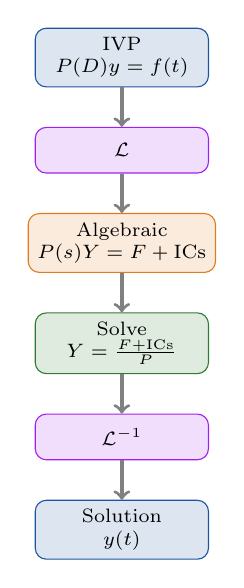
\begin{tikzpicture}[scale=0.55, node distance=5mm]
\tikzset{box/.style={draw, rounded corners, minimum width=2.2cm, minimum height=0.58cm, align=center, font=\scriptsize}}
\node[box, fill=headerblue!15, draw=headerblue] (ivp) {IVP\\$P(D)y = f(t)$};
\node[box, fill=workpurple!15, draw=workpurple, below=of ivp] (lap) {$\mathcal{L}$};
\node[box, fill=accentorange!15, draw=accentorange, below=of lap] (alg) {Algebraic\\$P(s)Y = F + \text{ICs}$};
\node[box, fill=accentgreen!15, draw=accentgreen, below=of alg] (sol) {Solve\\$Y = \frac{F+\text{ICs}}{P}$};
\node[box, fill=workpurple!15, draw=workpurple, below=of sol] (inv) {$\mathcal{L}^{-1}$};
\node[box, fill=headerblue!15, draw=headerblue, below=of inv] (ans) {Solution\\$y(t)$};
\draw[->, very thick, gray] (ivp) -- (lap);
\draw[->, very thick, gray] (lap) -- (alg);
\draw[->, very thick, gray] (alg) -- (sol);
\draw[->, very thick, gray] (sol) -- (inv);
\draw[->, very thick, gray] (inv) -- (ans);
\end{tikzpicture}
\end{column}
\end{columns}
\end{frame}

% ─── Slide 23 (cont.): Five-Step rationale ───
\begin{frame}{The Five-Step Laplace Method (cont.)}
\footnotesize
\begin{conceptbox}[Why This Beats Classical Methods]
\begin{itemize}
\item Initial conditions are absorbed automatically.
\item Discontinuous and impulsive forcing are handled natively.
\item The $s$-domain form exposes the structure of the solution.
\end{itemize}
\end{conceptbox}
\end{frame}

% ─── Slide 24: Homogeneous ODEs ───
\begin{frame}{Homogeneous ODEs --- Three Examples}
\footnotesize
\begin{columns}[T]
\begin{column}{0.32\textwidth}
\begin{examplebox}[Distinct Real Roots]
\textbf{Problem.} $y'' - 5y' + 6y = 0$, $y(0)=1, y'(0)=3$.

Transform: $(s^2-5s+6)Y = s-2$.
\resizeeq{Y = \frac{s-2}{(s-2)(s-3)} = \frac{1}{s-3}}
\textbf{Answer:} $y(t) = e^{3t}$.
\end{examplebox}
\end{column}
\begin{column}{0.32\textwidth}
\begin{examplebox}[Repeated Roots]
\textbf{Problem.} $y'' + 2y' + y = 0$, $y(0)=1, y'(0)=0$.

Transform: $(s+1)^2 Y = s + 2$.
\resizeeq{Y = \frac{s+2}{(s+1)^2} = \frac{1}{s+1} + \frac{1}{(s+1)^2}}
\textbf{Answer:} $y(t) = (1+t)e^{-t}$.
\end{examplebox}
\end{column}
\begin{column}{0.32\textwidth}
\begin{examplebox}[Complex Roots]
\textbf{Problem.} $y'' + 4y = 0$, $y(0)=2, y'(0)=3$.

Transform: $(s^2+4)Y = 2s+3$.
\resizeeq{Y = \frac{2s}{s^2+4} + \frac{3}{s^2+4}}
\textbf{Answer:} $y(t) = 2\cos(2t) + \tfrac{3}{2}\sin(2t)$.
\end{examplebox}
\end{column}
\end{columns}
\vspace{1mm}
\begin{conceptbox}[Pattern]
Each case reduces to factoring the characteristic polynomial in $s$, partial fractions, and table lookup. The Laplace method handles all three cases uniformly.
\end{conceptbox}
\end{frame}

% ─── Slide 25: Forced Oscillation ───
\begin{frame}{Forced Oscillation --- Two Examples}
\footnotesize
\begin{columns}[T]
\begin{column}{0.48\textwidth}
\begin{examplebox}[Sinusoidal Forcing]
\textbf{Problem.} $y'' + 4y = 3\cos t$, $y(0)=y'(0)=0$.

Transform: $(s^2+4)Y = \frac{3s}{s^2+1}$.
\[Y = \frac{3s}{(s^2+1)(s^2+4)} = \frac{s}{s^2+1} - \frac{s}{s^2+4}\]
\textbf{Answer:} $y(t) = \cos t - \cos(2t)$.
\end{examplebox}
\end{column}
\begin{column}{0.48\textwidth}
\begin{examplebox}[Exponential Forcing]
\textbf{Problem.} $y' - 2y = e^{5t}$, $y(0)=3$.

Transform: $(s-2)Y - 3 = \frac{1}{s-5}$.
\[Y = \frac{3s-14}{(s-5)(s-2)} = \frac{1/3}{s-5} + \frac{8/3}{s-2}\]
\textbf{Answer:} $y(t) = \tfrac{1}{3}e^{5t} + \tfrac{8}{3}e^{2t}$.
\end{examplebox}
\end{column}
\end{columns}
\vspace{1mm}
\begin{conceptbox}[Key Takeaway]
Both examples reduce to factoring a polynomial in $s^2$ (or $s$), partial fractions, and table lookup. The Laplace method sidesteps the classical ``particular + homogeneous'' decomposition.
\end{conceptbox}
\end{frame}

% ─── Slide 26: Discontinuous Forcing ───
\begin{frame}{Discontinuous Forcing --- Heaviside in Action}
\footnotesize
\begin{examplebox}[A Mass-Spring Switched Off at $t=7$]
\textbf{Problem.} $y'' + 2y' + 5y = h(t)$, $y(0)=y'(0)=0$, where $h(t) = 5$ for $t < 7$ and $0$ for $t > 7$. Equivalently: $h(t) = 5(1 - u_7(t))$.

\textbf{Step 1.} Transform (using $\mathcal{L}\{1\} = 1/s$ and $\mathcal{L}\{u_7\} = e^{-7s}/s$):
\[(s^2 + 2s + 5)\,Y = \frac{5}{s} - \frac{5e^{-7s}}{s}\]

\textbf{Step 2.} Solve:
\[Y(s) = \frac{5}{s(s^2+2s+5)} - \frac{5e^{-7s}}{s(s^2+2s+5)}\]
\end{examplebox}
\end{frame}

% ─── Slide 26 (cont.): Discontinuous Forcing --- decompose & invert ───
\begin{frame}{Discontinuous Forcing --- Heaviside in Action (cont.)}
\footnotesize
\begin{examplebox}[A Mass-Spring Switched Off at $t=7$ (cont.)]
\textbf{Step 3.} Decompose the first term:
\[\frac{5}{s(s^2+2s+5)} = \frac{1}{s} - \frac{s+2}{(s+1)^2+4}\]

Complete the square: $(s+1)^2 + 4 = (s+1)^2 + 2^2$.
\[\mathcal{L}^{-1}\!\left\{\frac{s+2}{(s+1)^2+4}\right\} = e^{-t}\cos(2t) + \tfrac{1}{2}e^{-t}\sin(2t)\]

\textbf{Step 4.} Apply the second shifting property to the $e^{-7s}$ term (delay by 7, zero before $t=7$).

\textbf{Answer:}
\begin{align*}
y(t) =\ & 1 - e^{-t}\cos(2t) - \tfrac{1}{2}e^{-t}\sin(2t) \\
& - u_7(t)\Big[1 - e^{-(t-7)}\cos(2(t-7)) - \tfrac{1}{2}e^{-(t-7)}\sin(2(t-7))\Big]
\end{align*}
\end{examplebox}
\end{frame}

% ─── Slide 26 (cont.): Discontinuous Forcing --- takeaways ───
\begin{frame}{Discontinuous Forcing --- Heaviside in Action (cont.)}
\footnotesize
\begin{conceptbox}[What Just Happened?]
A single Laplace-transform equation handled \emph{both regimes} of the forcing (on for $t<7$, off for $t>7$) in one algebraic expression. The classical method would require solving \emph{two separate IVPs} and stitching the solutions by enforcing continuity at $t=7$.
\end{conceptbox}
\vspace{0.5mm}
\begin{warningbox}[Common Pitfall]
When applying the second shifting property to $e^{-7s}F(s)$, the inverse $f(t)$ must be expressed in terms of $t$, then replaced by $t \to t-7$ and multiplied by $u_7(t)$. Forgetting the $u_7$ factor is the most common mistake.
\end{warningbox}
\end{frame}

% ─── Slide 27: Impulse Forcing ───
\begin{frame}{Impulse Forcing --- A Hammer Strike at $t=4$}
\footnotesize
\begin{columns}[T]
\begin{column}{0.58\textwidth}
\begin{examplebox}[Damped Oscillator Struck at $t=4$]
\textbf{Problem.} $y'' + 2y' + 26y = \delta_4(t)$, $y(0)=1, y'(0)=0$.

\textbf{Step 1.} Transform (using $\mathcal{L}\{\delta_4\} = e^{-4s}$):
\[[s^2Y - s] + 2[sY - 2] + 26Y = e^{-4s}\]

\textbf{Step 2.} Solve:
\[Y(s) = \frac{s+2}{(s+1)^2+25} + \frac{e^{-4s}}{(s+1)^2+25}\]
\end{examplebox}
\end{column}
\begin{column}{0.38\textwidth}
\centering
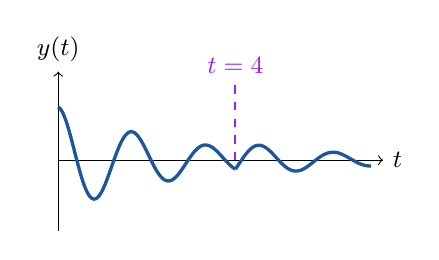
\begin{tikzpicture}[scale=0.75]
\draw[->] (0,0) -- (5.5,0) node[right] {\small $t$};
\draw[->] (0,-1.2) -- (0,1.5) node[above] {\small $y(t)$};
\draw[dashed, workpurple, thick] (3,0) -- (3,1.3);
\node[workpurple, above] at (3,1.3) {\small $t=4$};
\draw[headerblue, very thick, domain=0:3, samples=80] plot (\x, {0.9*exp(-0.5*\x)*cos(5*\x r)});
\draw[headerblue, very thick, domain=3:5.3, samples=120] plot (\x, {0.9*exp(-0.5*\x)*cos(5*\x r) + 0.4*exp(-0.5*(\x-3))*sin(5*(\x-3) r)});
\end{tikzpicture}\\[1mm]
{\footnotesize\color{headerblue}Damped oscillation; new mode appears at $t=4$}
\vspace{1mm}
\begin{conceptbox}[Key Takeaway]
An impulse $\delta_a(t)$ produces $e^{-as}H(s)$ in $Y(s)$, which inverts to $u_a(t)\,h(t-a)$ --- the impulse response delayed by $a$. The system ``remembers'' the impulse forever.
\end{conceptbox}
\end{column}
\end{columns}
\end{frame}

% ─── Slide 27 (cont.): Impulse Forcing --- split & invert ───
\begin{frame}{Impulse Forcing --- A Hammer Strike at $t=4$ (cont.)}
\footnotesize
\begin{examplebox}[Damped Oscillator Struck at $t=4$ (cont.)]
\textbf{Step 3.} Split the first term:
\[\frac{s+2}{(s+1)^2+25} = \frac{s+1}{(s+1)^2+5^2} + \frac{1}{5}\cdot\frac{5}{(s+1)^2+5^2}\]
Invert: $e^{-t}\cos(5t) + \tfrac{1}{5}e^{-t}\sin(5t)$.

\textbf{Step 4.} For the $e^{-4s}$ term, apply the second shifting property:
\[\mathcal{L}^{-1}\!\left\{\frac{e^{-4s}}{(s+1)^2+25}\right\} = u_4(t)\cdot\tfrac{1}{5}e^{-(t-4)}\sin(5(t-4))\]

\textbf{Answer:}
\begin{align*}
y(t) =\ & e^{-t}\cos(5t) + \tfrac{1}{5}e^{-t}\sin(5t) \\
& + u_4(t)\cdot\tfrac{1}{5}e^{-(t-4)}\sin(5(t-4))
\end{align*}
The third term is a new oscillation that switches on at $t=4$ --- the impulse response.
\end{examplebox}
\end{frame}

% ─── Slide 28: Periodic Forcing ───
\begin{frame}{Periodic Functions and Their Transforms}
\footnotesize
\begin{columns}[T]
\begin{column}{0.42\textwidth}
\begin{formulabox}[Periodic Function Transform]
If $f$ has period $P$ (i.e., $f(t+P) = f(t)$):
\[\mathcal{L}\{f(t)\} = \frac{1}{1 - e^{-Ps}} \int_0^P e^{-st}\, f(t)\, dt\]
\end{formulabox}
\vspace{0.5mm}
\begin{methodbox}[Proof Sketch]
Split $\int_0^{\infty} = \int_0^P + \int_P^{2P} + \cdots$. By periodicity, the $k$-th integral equals $e^{-kPs}\!\int_0^P\! e^{-st}f(t)\,dt$. Sum the geometric series $\sum e^{-kPs} = 1/(1-e^{-Ps})$.
\end{methodbox}
\end{column}
\begin{column}{0.56\textwidth}
\begin{examplebox}[Square Wave]
$f(t) = +1$ on $[0,2)$, $-1$ on $[2,4)$, period $P=4$.
\begin{align*}
\int_0^4 e^{-st}f(t)\,dt &= \int_0^2\! e^{-st}dt - \int_2^4\! e^{-st}dt \\
&= \frac{(1-e^{-2s})^2}{s}
\end{align*}
\[F(s) = \frac{(1-e^{-2s})^2}{s(1-e^{-4s})} = \frac{1-e^{-2s}}{s(1+e^{-2s})}\]
using $1-e^{-4s} = (1-e^{-2s})(1+e^{-2s})$.
\end{examplebox}
\vspace{0.5mm}
\begin{examplebox}[Sawtooth Wave]
$f(t) = t$ on $[0,1)$, period $P=1$. After integration by parts:
\[F(s) = \frac{1}{s^2} - \frac{e^{-s}}{s(1-e^{-s})}\]
\end{examplebox}
\end{column}
\end{columns}
\end{frame}

% ─── Slide 29: Linear Systems ───
\begin{frame}{Solving Linear Systems with Laplace}
\footnotesize
\begin{columns}[T]
\begin{column}{0.38\textwidth}
\begin{methodbox}[The Method]
For a system
\begin{align*}
a_1 x' + a_2 y' + a_3 x + a_4 y &= \beta_1(t) \\
b_1 x' + b_2 y' + b_3 x + b_4 y &= \beta_2(t)
\end{align*}
\begin{enumerate}
\item Transform each equation: $x' \to sX - x(0)$, $y' \to sY - y(0)$, $x \to X$, $y \to Y$.
\item The result is a $2\times 2$ linear algebraic system in $X(s), Y(s)$.
\item Solve by elimination or Cramer's rule.
\item Apply partial fractions and invert.
\end{enumerate}
\end{methodbox}
\end{column}
\begin{column}{0.6\textwidth}
\begin{examplebox}[Worked Example]
\textbf{System:} $x' - 6x + 3y = 8e^t$, $y' - 2x - y = 4e^t$, with $x(0)=-1, y(0)=0$.

Transform both equations:
\begin{align*}
(sX+1) - 6X + 3Y &= \frac{8}{s-1} \\
sY - 2X - Y &= \frac{4}{s-1}
\end{align*}
Rearrange:
\begin{align*}
(s-6)X + 3Y &= \frac{-s+9}{s-1} \\
-2X + (s-1)Y &= \frac{4}{s-1}
\end{align*}
\end{examplebox}
\end{column}
\end{columns}
\end{frame}

% ─── Slide 29 (cont.): Linear Systems --- solve & invert ───
\begin{frame}{Solving Linear Systems with Laplace (cont.)}
\footnotesize
\begin{examplebox}[Worked Example (cont.)]
Solve (Cramer's rule):
\[X(s) = \frac{-s+7}{(s-1)(s-4)}, \quad Y(s) = \frac{2}{(s-1)(s-4)}\]
Partial fractions and invert:
\[x(t) = -2e^t + e^{4t}, \quad y(t) = -\tfrac{2}{3}e^t + \tfrac{2}{3}e^{4t}\]
\end{examplebox}
\end{frame}

% ─── Slide 29 (cont.): Linear Systems takeaway ───
\begin{frame}{Solving Linear Systems with Laplace (cont.)}
\footnotesize
\begin{conceptbox}[Key Takeaway]
The Laplace method scales effortlessly to systems --- the algebraic structure in $s$ is what would be obtained by diagonalizing the coefficient matrix, but the ICs are incorporated from the start.
\end{conceptbox}
\end{frame}

% ─── Slide 30: Inverse Laplace Techniques ───
\begin{frame}{Inverse Laplace --- The Four Techniques}
\footnotesize
\centering
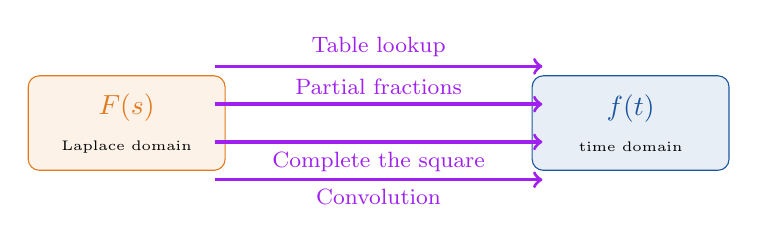
\begin{tikzpicture}[scale=0.8]
\node[draw=accentorange, fill=accentorange!10, rounded corners, minimum width=2.5cm, minimum height=1.2cm, align=center] at (0,0) {\textbf{\color{accentorange}$F(s)$}\\[1pt]\tiny Laplace domain};
\node[draw=headerblue, fill=headerblue!10, rounded corners, minimum width=2.5cm, minimum height=1.2cm, align=center] at (8,0) {\textbf{\color{headerblue}$f(t)$}\\[1pt]\tiny time domain};
\draw[->, workpurple, very thick] (1.4,0.3) -- (6.6,0.3);
\draw[->, workpurple, very thick] (1.4,-0.3) -- (6.6,-0.3);
\draw[->, workpurple, very thick] (1.4,0.9) -- (6.6,0.9);
\draw[->, workpurple, very thick] (1.4,-0.9) -- (6.6,-0.9);
\node[workpurple, above] at (4,0.9) {\footnotesize Table lookup};
\node[workpurple, above] at (4,0.3) {\footnotesize Partial fractions};
\node[workpurple, below] at (4,-0.3) {\footnotesize Complete the square};
\node[workpurple, below] at (4,-0.9) {\footnotesize Convolution};
\end{tikzpicture}
\vspace{1mm}
\begin{columns}[T]
\begin{column}{0.48\textwidth}
\begin{methodbox}[Technique 1 --- Table Lookup]
Memorize the six starter transforms. Add shifting properties for $(s-a)$ patterns, derivative rules for ODEs. Most problems reduce to this.

\medskip
\emph{Example:} $\mathcal{L}^{-1}\!\left\{\frac{3}{s^2+9}\right\} = \sin(3t)$.
\end{methodbox}
\end{column}
\begin{column}{0.48\textwidth}
\begin{methodbox}[Technique 2 --- Partial Fractions]
For rational $F(s) = N(s)/D(s)$ with $\deg N < \deg D$, factor $D(s)$ and decompose. Distinct linear $\to \sum A_k/(s-r_k)$; repeated $\to \sum A_k/(s-r)^k$; irreducible quadratics $\to (Bs+C)/(s^2+bs+c)$.

\medskip
\emph{Example:} $\frac{3s-14}{(s-5)(s-2)} = \frac{1/3}{s-5} + \frac{8/3}{s-2} \to \tfrac{1}{3}e^{5t}+\tfrac{8}{3}e^{2t}$.
\end{methodbox}
\end{column}
\end{columns}
\end{frame}

% ─── Slide 30 (cont.): inverse-Laplace techniques 3 & 4 ───
\begin{frame}{Inverse Laplace --- The Four Techniques (cont.)}
\footnotesize
\begin{columns}[T]
\begin{column}{0.48\textwidth}
\begin{methodbox}[Technique 3 --- Complete the Square]
For irreducible $s^2+bs+c$, rewrite as $(s+b/2)^2 + (c-b^2/4)$. Match to $\frac{s+a}{(s+a)^2+\omega^2}$ (cosine) or $\frac{\omega}{(s+a)^2+\omega^2}$ (sine); first shifting gives $e^{-at}$.

\medskip
\emph{Example:} $\frac{1}{s^2+6s+13} = \frac{1}{(s+3)^2+4} \to \tfrac{1}{2}e^{-3t}\sin(2t)$.
\end{methodbox}
\end{column}
\begin{column}{0.48\textwidth}
\begin{methodbox}[Technique 4 --- Convolution]
For products $F(s)G(s)$ resisting partial fractions:
\[\mathcal{L}^{-1}\{FG\} = f * g = \int_0^t f(\tau)\,g(t-\tau)\,d\tau\]
\emph{Example:} $\mathcal{L}^{-1}\!\left\{\frac{1}{s^2(s+1)}\right\} = t * e^{-t} = t + e^{-t} - 1$.
\end{methodbox}
\end{column}
\end{columns}
\end{frame}

% ─── Slide 31: Mass-Spring-Dashpot ───
\begin{frame}{The Mass-Spring-Dashpot System}
\footnotesize
\begin{columns}[T]
\begin{column}{0.38\textwidth}
\centering
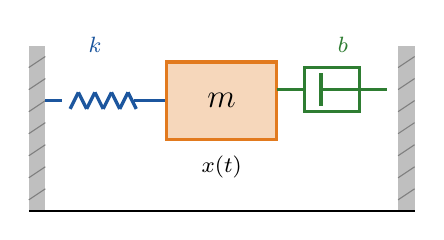
\begin{tikzpicture}[scale=0.7]
% Wall
\fill[gray!50] (0,0.5) rectangle (0.3,3.5);
\foreach \y in {0.7,1.1,1.5,1.9,2.3,2.7,3.1} \draw[gray] (0,\y) -- (0.3,\y+0.2);
% Spring
\draw[headerblue, very thick] (0.3,2.5) -- (0.6,2.5);
\foreach \i in {1,...,8} \draw[headerblue, very thick] ({0.6+0.15*\i}, {2.5+0.15*((-1)^\i)}) -- ({0.6+0.15*(\i+1)}, {2.5+0.15*((-1)^(\i+1))});
\draw[headerblue, very thick] (1.9,2.5) -- (2.5,2.5);
% Mass
\draw[fill=accentorange!30, draw=accentorange, very thick] (2.5,1.8) rectangle (4.5,3.2);
\node at (3.5,2.5) {\large $m$};
% Dashpot
\draw[accentgreen, very thick] (4.5,2.7) -- (5.0,2.7);
\draw[accentgreen, very thick] (5.0,2.3) rectangle (6.0,3.1);
\draw[accentgreen, very thick] (5.3,2.4) -- (5.3,3.0);
\draw[accentgreen, very thick] (5.3,2.7) -- (6.5,2.7);
% Right wall
\fill[gray!50] (6.7,0.5) rectangle (7,3.5);
\foreach \y in {0.7,1.1,1.5,1.9,2.3,2.7,3.1} \draw[gray] (6.7,\y) -- (7,\y+0.2);
% Ground
\draw[thick] (0,0.5) -- (7,0.5);
\node[headerblue, above] at (1.2,3.2) {\footnotesize $k$};
\node[accentgreen, above] at (5.7,3.2) {\footnotesize $b$};
\node at (3.5,1.3) {\footnotesize $x(t)$};
\end{tikzpicture}
\vspace{0.5mm}
\begin{formulabox}[The ODE]
\[mx'' + bx' + kx = f(t)\]
$x(0) = x_0, \quad x'(0) = v_0$
\end{formulabox}
\end{column}
\begin{column}{0.58\textwidth}
\begin{methodbox}[General Solution via Laplace]
Transform: $m(s^2X - sx_0 - v_0) + b(sX - x_0) + kX = F(s)$. Solve:
\[X(s) = \frac{F(s) + m(x_0 s + v_0) + b\,x_0}{ms^2 + bs + k}\]
The denominator $ms^2 + bs + k$ is the \emph{characteristic polynomial}. Its roots determine the homogeneous behavior (overdamped, critically damped, underdamped).
\end{methodbox}
\end{column}
\end{columns}
\end{frame}

% ─── Slide 31 (cont.): Mass-Spring --- forced motion & takeaway ───
\begin{frame}{The Mass-Spring-Dashpot System (cont.)}
\footnotesize
\begin{examplebox}[Forced Undamped Motion]
$x'' + 4x = \sin(3t)$, $x(0) = x'(0) = 0$. Transform:
\[(s^2+4)X = \frac{3}{s^2+9} \;\Rightarrow\; X = \frac{3}{(s^2+4)(s^2+9)}\]
Partial fractions:
\[\frac{3}{(s^2+4)(s^2+9)} = \frac{3/5}{s^2+4} - \frac{3/5}{s^2+9}\]
Invert: $x(t) = \tfrac{3}{10}\sin(2t) - \tfrac{1}{5}\sin(3t)$.

A superposition of two oscillations --- natural frequency $2$ and forcing frequency $3$. No resonance.
\end{examplebox}
\vspace{0.5mm}
\begin{conceptbox}[Key Takeaway]
The Laplace method gives the full solution --- homogeneous + particular + ICs --- in one algebraic equation. The denominator reveals the natural frequencies; the numerator reveals the forcing response.
\end{conceptbox}
\end{frame}

% ═══════════════════════════════════════════════════════════════════
% PART IV --- CONVOLUTION & SYSTEMS
% ═══════════════════════════════════════════════════════════════════

\section{Part IV --- Convolution \& Systems}

% ─── Slide 32: Section Header Part IV ───
{
\setbeamercolor{background canvas}{bg=headerblue}
\setbeamertemplate{footline}{}
\begin{frame}[plain]
\vspace{2cm}
{\color{accentorange}\Huge\textbf{PART IV}}\\[0.4cm]
{\color{white}\Huge\textbf{Convolution \& Systems}}\\[0.8cm]
{\color{white!85}\large The convolution theorem. Duhamel's principle. Volterra equations.\\
Transfer functions. Impulse response. Poles, zeros, and stability.}
\end{frame}
}

% ─── Slide 33: Convolution Theorem ───
\begin{frame}{The Convolution Theorem}
\footnotesize
\begin{columns}[T]
\begin{column}{0.42\textwidth}
\begin{formulabox}[Definition and Theorem]
\textbf{Convolution:}
\resizeeq{(f * g)(t) = \int_0^t f(\tau)\,g(t-\tau)\,d\tau = \int_0^t f(t-\tau)\,g(\tau)\,d\tau}
The two forms are equal (substitute $u = t-\tau$).

\medskip
\textbf{Convolution Theorem:}
\[\mathcal{L}\{f * g\} = \mathcal{L}\{f\}\cdot\mathcal{L}\{g\} = F(s)\,G(s)\]
\[\mathcal{L}^{-1}\{F(s)\,G(s)\} = (f * g)(t)\]
\end{formulabox}
\end{column}
\begin{column}{0.56\textwidth}
\begin{methodbox}[Proof Sketch --- the geometric version]
Write the product $F(s)\,G(s)$ as a double integral over the first quadrant:
\[F(s)\,G(s) = \int_0^{\infty}\!\!\int_0^{\infty} e^{-s(u+v)} f(u)\,g(v)\,du\,dv\]
Change variables: $t = u+v$, $\tau = v$ (Jacobian $= 1$). The first quadrant becomes the wedge $0 \le \tau \le t < \infty$. Swap the order of integration:
\resizeeq{F(s)\,G(s) = \int_0^{\infty} e^{-st}\!\left[\int_0^t f(t-\tau)\,g(\tau)\,d\tau\right]dt = \mathcal{L}\{f * g\}}
\end{methodbox}
\vspace{0.5mm}
\begin{conceptbox}[Key Takeaway]
The convolution theorem is the \emph{product rule} for Laplace transforms. It converts products in the $s$-domain into convolutions in the $t$-domain. This is the foundation for transfer functions and Duhamel's principle.
\end{conceptbox}
\end{column}
\end{columns}
\end{frame}

% ─── Slide 34: Convolution Properties ───
\begin{frame}{Convolution: Properties and Pitfalls}
\footnotesize
\begin{columns}[T]
\begin{column}{0.48\textwidth}
\begin{methodbox}[Algebraic Properties]
For piecewise-continuous exponentially-bounded $f, g, h$ and constant $c$:
\begin{itemize}
\item \textbf{Commutative:} $f * g = g * f$
\item \textbf{Associative:} $f * (g * h) = (f * g) * h$
\item \textbf{Distributive:} $f * (g + h) = f * g + f * h$
\item \textbf{Scalar:} $(cf) * g = c(f * g)$
\item \textbf{Zero:} $0 * f = f * 0 = 0$
\end{itemize}
\end{methodbox}
\end{column}
\begin{column}{0.48\textwidth}
\begin{warningbox}[CRITICAL: No Multiplicative Identity]
$f * 1 \ne f$. The function $1$ is \emph{not} the identity for convolution. For example, $(\cos t) * 1 = \sin t$, \emph{not} $\cos t$.

\medskip
The identity for convolution is the Dirac delta: $(f * \delta)(t) = f(t)$. This is the sifting property.
\end{warningbox}
\vspace{0.5mm}
\begin{warningbox}[Pitfall 2 --- $f * f$ not non-negative]
Unlike $f(t)^2$, the convolution $f * f$ can be negative. For example, $(\sin t) * (\sin t) = \tfrac{1}{2}(\sin t - t\cos t)$, which is negative on intervals.
\end{warningbox}
\end{column}
\end{columns}
\end{frame}

% ─── Slide 34 (cont.): convolution worked example ───
\begin{frame}{Convolution: Properties and Pitfalls (cont.)}
\footnotesize
\begin{examplebox}[$(\cos t) * (\cos t)$]
Use $\cos(t-\tau)\cos\tau = \tfrac{1}{2}[\cos(t-2\tau) + \cos t]$:
\[\begin{aligned}
(\cos * \cos)(t) &= \int_0^t \cos(t-\tau)\cos\tau\,d\tau \\
&= \tfrac{1}{2}\int_0^t [\cos(t-2\tau)+\cos t]\,d\tau \\
&= \tfrac{1}{2}[\sin t + t\cos t]
\end{aligned}\]
\end{examplebox}
\end{frame}

% ─── Slide 35: Duhamel's Principle ───
\begin{frame}{Duhamel's Principle --- Solution for Arbitrary Input}
\footnotesize
\begin{columns}[T]
\begin{column}{0.58\textwidth}
\begin{examplebox}[The Killer Application]
\textbf{Problem.} Solve $x'' + \omega_0^2\, x = f(t)$, $x(0) = x'(0) = 0$, for \emph{arbitrary} $f(t)$.

\textbf{Step 1.} Transform: $s^2 X + \omega_0^2 X = F(s)$, so
\[X(s) = \frac{F(s)}{s^2 + \omega_0^2}\]

\textbf{Step 2.} Recognize $\frac{1}{s^2+\omega_0^2}$ as the \emph{transfer function} $H(s)$, with inverse $h(t) = \frac{\sin(\omega_0 t)}{\omega_0}$.

\textbf{Step 3.} Apply the convolution theorem: $X(s) = H(s)\,F(s)$ implies
\[x(t) = (h * f)(t) = \int_0^t \frac{\sin(\omega_0(t-\tau))}{\omega_0}\, f(\tau)\,d\tau\]

\end{examplebox}
\end{column}
\begin{column}{0.38\textwidth}
\centering
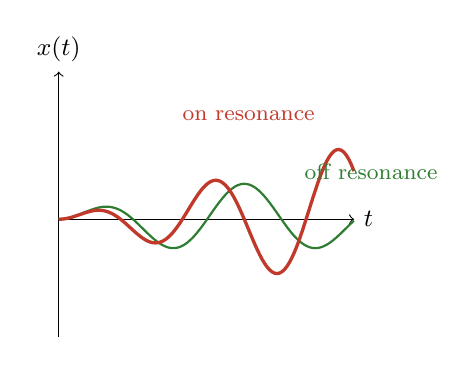
\begin{tikzpicture}[scale=0.75]
\draw[->] (0,0) -- (5,0) node[right] {\small $t$};
\draw[->] (0,-2) -- (0,2.5) node[above] {\small $x(t)$};
\draw[accentgreen, thick, domain=0:5, samples=100] plot (\x, {0.3*cos(2*\x r) - 0.3*cos(3*\x r)});
\draw[warnred, very thick, domain=0:5, samples=120] plot (\x, {0.25*\x*sin(3*\x r)});
\node[accentgreen, above right] at (4,0.5) {\footnotesize off resonance};
\node[warnred, above left] at (4.5,1.5) {\footnotesize on resonance};
\end{tikzpicture}\\[1mm]
{\footnotesize\color{warnred}Resonance: amplitude grows linearly}
\vspace{1mm}
\begin{conceptbox}[Key Takeaway]
Once the impulse response $h(t)$ of a system is known, its response to \emph{any} input is the convolution with $h$. The system is fully characterized by $h$.
\end{conceptbox}
\end{column}
\end{columns}
\end{frame}

% ─── Slide 35 (cont.): Duhamel --- resonance check ───
\begin{frame}{Duhamel's Principle --- Solution for Arbitrary Input (cont.)}
\footnotesize
\begin{examplebox}[The Killer Application (cont.)]
\textbf{Step 4.} Resonance check: if $f(t) = \cos(\omega_0 t)$, the convolution evaluates to
\[x(t) = \frac{t\,\sin(\omega_0 t)}{2\omega_0}\]
--- the linearly-growing amplitude that defines \emph{resonance}.
\end{examplebox}
\end{frame}

% ─── Slide 36: Volterra Integral Equations ───
\begin{frame}{Volterra Integral Equations}
\footnotesize
\begin{columns}[T]
\begin{column}{0.42\textwidth}
\begin{formulabox}[The Volterra Equation]
\[x(t) = f(t) + \int_0^t g(t-\tau)\, x(\tau)\, d\tau\]
The unknown $x$ appears under the integral --- but the integral is a convolution $(g * x)(t)$. Apply $\mathcal{L}$:
\[X(s) = F(s) + G(s)\,X(s)\]
\[\Rightarrow\; X(s) = \frac{F(s)}{1 - G(s)}\]
Pure algebra. Then invert $X(s)$.
\end{formulabox}
\end{column}
\begin{column}{0.56\textwidth}
\begin{examplebox}[Worked Example]
\textbf{Equation:} $x(t) = e^{-t} + \int_0^t \sinh(t-\tau)\, x(\tau)\, d\tau$.

Transform (using $\mathcal{L}\{e^{-t}\} = \frac{1}{s+1}$ and $\mathcal{L}\{\sinh t\} = \frac{1}{s^2-1}$):
\[X = \frac{1}{s+1} + \frac{1}{s^2-1}\,X\]
Solve:
\[X\!\left(1 - \frac{1}{s^2-1}\right) = \frac{1}{s+1} \;\Rightarrow\; X\cdot\frac{s^2-2}{s^2-1} = \frac{1}{s+1}\]
\[X = \frac{s^2-1}{(s+1)(s^2-2)} = \frac{s-1}{s^2-2}\]
using $s^2-1 = (s-1)(s+1)$.
\end{examplebox}
\end{column}
\end{columns}
\end{frame}

% ─── Slide 36 (cont.): Volterra --- decompose & invert ───
\begin{frame}{Volterra Integral Equations (cont.)}
\footnotesize
\begin{examplebox}[Worked Example (cont.)]
Decompose: $\frac{s-1}{s^2-2} = \frac{s}{s^2-2} - \frac{1}{s^2-2}$. Recognize:
\[\mathcal{L}^{-1}\!\left\{\frac{s}{s^2-2}\right\} = \cosh(\sqrt{2}\,t), \quad \mathcal{L}^{-1}\!\left\{\frac{1}{s^2-2}\right\} = \frac{1}{\sqrt{2}}\sinh(\sqrt{2}\,t)\]
\textbf{Answer:} $x(t) = \cosh(\sqrt{2}\,t) - \frac{1}{\sqrt{2}}\sinh(\sqrt{2}\,t)$.
\end{examplebox}
\vspace{0.5mm}
\begin{conceptbox}[Why This Matters]
Integral equations arise in physics problems with memory: viscoelastic materials, population models with age structure, radiative transfer. Laplace transforms solve them as cleanly as differential equations.
\end{conceptbox}
\end{frame}

% ─── Slide 37: Transfer Functions ───
\begin{frame}{Transfer Functions $H(s)$}
\footnotesize
\begin{columns}[T]
\begin{column}{0.58\textwidth}
\begin{formulabox}[Definition]
For a linear constant-coefficient ODE $P(D)\,x = N(D)\,E(t)$ with \emph{rest} initial conditions ($x(0) = x'(0) = \cdots = 0$):
\[H(s) = \frac{\mathcal{L}\{x\}}{\mathcal{L}\{E\}} = \frac{N(s)}{P(s)} = \frac{b_m s^m + \cdots + b_0}{a_n s^n + \cdots + a_0}\]
$H(s)$ depends \emph{only on the system}, not on the input. Once $H$ is known, the output for any input is $X(s) = H(s)\,E(s)$.
\end{formulabox}
\end{column}
\begin{column}{0.38\textwidth}
\centering
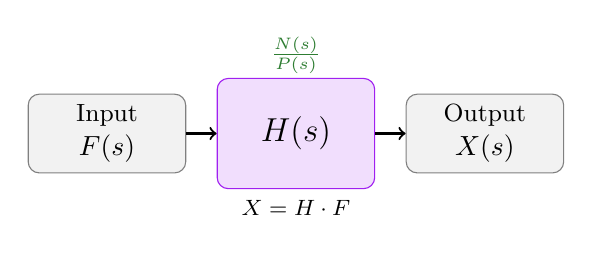
\begin{tikzpicture}[scale=0.8]
\node[draw=gray, fill=gray!10, rounded corners, minimum width=2cm, minimum height=1cm, align=center] (in) at (0,0) {\small Input\\$F(s)$};
\node[draw=workpurple, fill=workpurple!15, rounded corners, minimum width=2cm, minimum height=1.4cm, align=center] (h) at (3,0) {\large $H(s)$};
\node[draw=gray, fill=gray!10, rounded corners, minimum width=2cm, minimum height=1cm, align=center] (out) at (6,0) {\small Output\\$X(s)$};
\draw[->, thick] (in) -- (h);
\draw[->, thick] (h) -- (out);
\node[below] at (3,-0.9) {\footnotesize $X = H \cdot F$};
\node[above, accentgreen] at (3,0.8) {\footnotesize $\frac{N(s)}{P(s)}$};
\end{tikzpicture}
\vspace{3mm}
\begin{conceptbox}[Key Takeaway]
A system \emph{is} its transfer function. Two systems with the same $H(s)$ are indistinguishable from their input-output behavior --- even if their internal structures differ.
\end{conceptbox}
\end{column}
\end{columns}
\end{frame}

% ─── Slide 37 (cont.): Transfer function example ───
\begin{frame}{Transfer Functions $H(s)$ (cont.)}
\footnotesize
\begin{methodbox}[Why It Matters]
\begin{itemize}
\item Characterizes the system independent of input.
\item Poles of $H$ (roots of $P$) determine natural frequencies and stability.
\item Zeros of $H$ (roots of $N$) determine which inputs are ``absorbed.''
\item Engineers measure $H(i\omega)$ (frequency response) experimentally.
\end{itemize}
\end{methodbox}
\vspace{0.5mm}
\begin{examplebox}[Mass-Spring with Base Excitation]
For $mx'' + bx' + kx = bE'(t) + kE(t)$:
\[H(s) = \frac{bs + k}{ms^2 + bs + k}\]
Poles at $s = \frac{-b \pm \sqrt{b^2-4mk}}{2m}$; zero at $s = -k/b$.
\end{examplebox}
\end{frame}

% ─── Slide 38: Impulse Response ───
\begin{frame}{The Impulse Response $h(t)$}
\footnotesize
\begin{columns}[T]
\begin{column}{0.42\textwidth}
\begin{formulabox}[Definition]
\[h(t) = \mathcal{L}^{-1}\{H(s)\}\]
--- the inverse Laplace transform of the transfer function. Equivalently: the solution to $Lh = \delta(t)$ with rest initial conditions.

\medskip
The equivalence holds because $\mathcal{L}\{\delta\} = 1$, so $X(s) = H(s)\cdot 1 = H(s)$, hence $x(t) = h(t)$.
\end{formulabox}
\end{column}
\begin{column}{0.56\textwidth}
\begin{examplebox}[Undamped Oscillator]
\textbf{Problem.} Find the impulse response of $x'' + \omega_0^2 x = \delta(t)$, $x(0) = x'(0) = 0$.

Transform: $(s^2 + \omega_0^2)X = 1$, so $X(s) = \frac{1}{s^2+\omega_0^2} = H(s)$. Invert:
\[h(t) = \frac{\sin(\omega_0 t)}{\omega_0}\]

\end{examplebox}
\end{column}
\end{columns}
\end{frame}

% ─── Slide 38 (cont.): apply h; indicial vs impulse ───
\begin{frame}{The Impulse Response $h(t)$ (cont.)}
\footnotesize
\begin{methodbox}[The Big Payoff]
For any input $f(t)$, the output is the convolution with $h$:
\[x(t) = (h * f)(t) = \int_0^t h(t-\tau)\, f(\tau)\, d\tau\]
This is the Duhamel / superposition formula. The system is fully characterized by its impulse response.
\end{methodbox}
\vspace{0.5mm}
\begin{examplebox}[Undamped Oscillator (cont.)]
Now use this $h$ to solve $x'' + \omega_0^2 x = f(t)$ for \emph{any} $f$:
\[x(t) = (h * f)(t) = \int_0^t \frac{\sin(\omega_0(t-\tau))}{\omega_0}\, f(\tau)\, d\tau\]
A single integral --- no ODE solving required.
\end{examplebox}
\end{frame}

% ─── Slide 38 (cont.): indicial vs impulse ───
\begin{frame}{The Impulse Response $h(t)$ (cont.)}
\footnotesize
\begin{conceptbox}[Indicial vs Impulse Response]
The \emph{indicial response} $A(t)$ (response to unit step $u(t)$) and the \emph{impulse response} $h(t)$ (response to $\delta(t)$) are related by $A'(t) = h(t)$, i.e., $A(t) = \int_0^t h(\tau)\,d\tau$. Both characterize the system; $h$ is more fundamental.
\end{conceptbox}
\end{frame}

% ─── Slide 39: Poles, Zeros & Stability ───
\begin{frame}{Poles, Zeros, and Stability}
\footnotesize
\begin{columns}[T]
\begin{column}{0.42\textwidth}
\begin{formulabox}[Definitions]
For $H(s) = N(s)/P(s)$ in \emph{reduced form}:
\begin{itemize}
\item \textbf{Poles:} roots of $P(s)$ --- where $H \to \infty$.
\item \textbf{Zeros:} roots of $N(s)$ --- where $H = 0$.
\end{itemize}
The poles are exactly the roots of the characteristic equation --- they determine the natural frequencies.
\end{formulabox}
\end{column}
\begin{column}{0.56\textwidth}
\centering
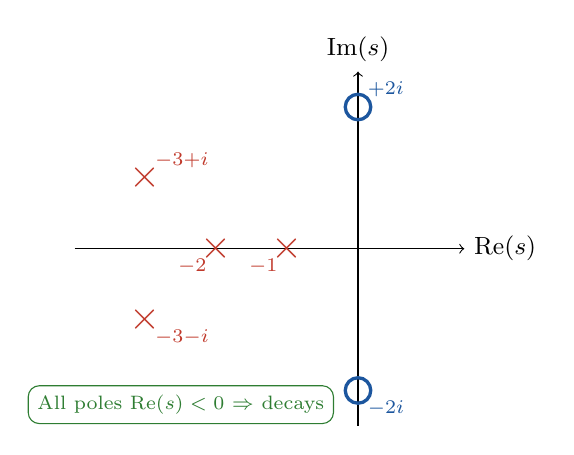
\begin{tikzpicture}[scale=0.9]
\draw[->] (-4,0) -- (1.5,0) node[right] {\small $\mathrm{Re}(s)$};
\draw[->] (0,-2.5) -- (0,2.5) node[above] {\small $\mathrm{Im}(s)$};
% Poles (red X)
\node[warnred, font=\Large] at (-1,0) {$\times$};
\node[warnred, font=\Large] at (-2,0) {$\times$};
\node[warnred, font=\Large] at (-3,1) {$\times$};
\node[warnred, font=\Large] at (-3,-1) {$\times$};
% Zeros (blue O)
\draw[headerblue, very thick] (0,2) circle (0.18);
\draw[headerblue, very thick] (0,-2) circle (0.18);
% Labels
\node[below left, warnred, font=\scriptsize] at (-1,0) {$-1$};
\node[below left, warnred, font=\scriptsize] at (-2,0) {$-2$};
\node[above right, warnred, font=\scriptsize] at (-3,1) {$-3{+}i$};
\node[below right, warnred, font=\scriptsize] at (-3,-1) {$-3{-}i$};
\node[above right, headerblue, font=\scriptsize] at (0,2) {$+2i$};
\node[below right, headerblue, font=\scriptsize] at (0,-2) {$-2i$};
% Stability note
\node[accentgreen, font=\scriptsize, draw=accentgreen, rounded corners, fill=white] at (-2.5,-2.2) {All poles $\mathrm{Re}(s)<0$ $\Rightarrow$ decays};
\end{tikzpicture}\\[2mm]
{\footnotesize Pole-zero plot: $H(s) = \frac{s^2+4}{(s^2+3s+2)(s^2+6s+10)}$}
\end{column}
\end{columns}
\end{frame}

% ─── Slide 39 (cont.): stability theorem & pitfall ───
\begin{frame}{Poles, Zeros, and Stability (cont.)}
\footnotesize
\begin{columns}[T]
\begin{column}{0.5\textwidth}
\begin{formulabox}[Stability Theorem]
For the homogeneous solution $x_h(t)$:
\begin{itemize}
\item $\mathrm{Re}(s_i) < 0$ for all poles $\Rightarrow$ $x_h \to 0$ exponentially (stable).
\item $\mathrm{Re}(s_i) > 0$ for any pole $\Rightarrow$ $x_h$ grows (unstable).
\item $\mathrm{Im}(s_i) \ne 0$ for any pole $\Rightarrow$ oscillations.
\item The rightmost pole dominates long-term behavior.
\end{itemize}
\end{formulabox}
\end{column}
\begin{column}{0.5\textwidth}
\begin{warningbox}[Common Pitfall]
A zero at $s = s_z$ means an input $e^{s_z t}$ produces no long-term response --- the system ``absorbs'' it. This is the principle behind notch filters.
\end{warningbox}
\end{column}
\end{columns}
\vspace{0.5mm}
\begin{conceptbox}[Key Takeaway]
The pole-zero plot is a complete picture of the system's natural behavior. Left half-plane $\to$ stable; imaginary axis $\to$ marginal; right half-plane $\to$ unstable.
\end{conceptbox}
\end{frame}

% ═══════════════════════════════════════════════════════════════════
% PART V --- ADVANCED APPLICATIONS
% ═══════════════════════════════════════════════════════════════════

\section{Part V --- Advanced Applications}

% ─── Slide 40: Section Header Part V ───
{
\setbeamercolor{background canvas}{bg=headerblue}
\setbeamertemplate{footline}{}
\begin{frame}[plain]
\vspace{2cm}
{\color{accentorange}\Huge\textbf{PART V}}\\[0.4cm]
{\color{white}\Huge\textbf{Advanced Applications}}\\[0.8cm]
{\color{white!85}\large PDEs via Laplace. Beam bending. Abel's tautochrone.\\
Real-integral tricks. Resonance. The transform's reach beyond ODEs.}
\end{frame}
}

% ─── Slide 41: Transport Equation ───
\begin{frame}{The Transport Equation via Laplace}
\footnotesize
\begin{columns}[T]
\begin{column}{0.58\textwidth}
\begin{examplebox}[River Pollution --- Wavefront at Speed $\alpha$]
\textbf{PDE.} $y_t = -\alpha\, y_x$ for $x > 0, t > 0$, with $y(0,t) = C$ and $y(x,0) = 0$. Here $\alpha > 0$ is the wave speed.

\textbf{Physical setup:} a river carrying toxic waste from a factory at $x=0$. The concentration at the factory is held at $C$; the river starts clean.

\textbf{Step 1.} Transform in $t$ (treat $x$ as a parameter). The PDE becomes an ODE in $x$:
\[s\, Y(x) = -\alpha\, Y'(x)\]

\textbf{Step 2.} Transform the BC $y(0,t) = C$: $Y(0) = C/s$.

\end{examplebox}
\end{column}
\begin{column}{0.38\textwidth}
\centering
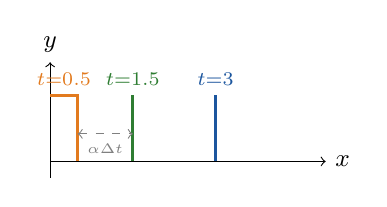
\begin{tikzpicture}[scale=0.7]
\draw[->] (0,0) -- (5,0) node[right] {\small $x$};
\draw[->] (0,-0.3) -- (0,1.8) node[above] {\small $y$};
\draw[accentorange, very thick] (0,1.2) -- (0.5,1.2) -- (0.5,0);
\draw[accentgreen, very thick] (1.5,1.2) -- (1.5,0);
\draw[headerblue, very thick] (3,1.2) -- (3,0);
\node[accentorange, above] at (0.25,1.2) {\scriptsize $t{=}0.5$};
\node[accentgreen, above] at (1.5,1.2) {\scriptsize $t{=}1.5$};
\node[headerblue, above] at (3,1.2) {\scriptsize $t{=}3$};
\draw[<->, dashed, gray] (0.5,0.5) -- (1.5,0.5);
\node[gray, below] at (1,0.5) {\tiny $\alpha\Delta t$};
\end{tikzpicture}\\[1mm]
{\footnotesize Wavefront travels at speed $\alpha$}
\vspace{1mm}
\begin{conceptbox}[Key Takeaway]
The Laplace transform reduces a PDE in two variables to an ODE in one by transforming one variable. The BC becomes the ODE's initial condition.
\end{conceptbox}
\end{column}
\end{columns}
\end{frame}

% ─── Slide 41 (cont.): transport --- solve & invert ───
\begin{frame}{The Transport Equation via Laplace (cont.)}
\footnotesize
\begin{examplebox}[River Pollution (cont.)]
\textbf{Step 3.} Solve the ODE:
\[Y(x) = \frac{C}{s}\, e^{-sx/\alpha}\]

\textbf{Step 4.} Invert using the second shifting property ($\mathcal{L}^{-1}\{\frac{1}{s}e^{-as}\} = u_a(t)$ with $a = x/\alpha$):
\[y(x,t) = C \cdot u(t - x/\alpha)\]
\end{examplebox}
\end{frame}

% ─── Slide 42: Heat Equation ───
\begin{frame}{The Heat Equation on a Half-Line}
\footnotesize
\begin{examplebox}[Half-Line with Prescribed Flux]
\textbf{PDE.} $y_t = y_{xx}$ for $x > 0, t > 0$, with $y_x(0,t) = f(t)$ (prescribed heat flux) and $y(x,0) = 0$, with $y$ bounded as $x \to \infty$.

\textbf{Step 1.} Transform in $t$: $sY = Y''$ --- an ODE in $x$.

\textbf{Step 2.} General solution: $Y(x) = A e^{\sqrt{s}\,x} + B e^{-\sqrt{s}\,x}$. Boundedness as $x \to \infty$ forces $A = 0$. So $Y(x) = B\, e^{-\sqrt{s}\,x}$.

\textbf{Step 3.} Apply the flux BC: $Y'(0) = -\sqrt{s}\, B = F(s)$, so $B = -F(s)/\sqrt{s}$. Hence
\[Y(x) = -\frac{F(s)}{\sqrt{s}}\, e^{-\sqrt{s}\,x}\]
\end{examplebox}
\end{frame}

% ─── Slide 42 (cont.): Heat Equation --- inversion ───
\begin{frame}{The Heat Equation on a Half-Line (cont.)}
\footnotesize
\begin{examplebox}[Half-Line with Prescribed Flux (cont.)]
\textbf{Step 4.} Use the table identity:
\[\mathcal{L}^{-1}\!\left\{\frac{1}{\sqrt{s}}\, e^{-\sqrt{s}\,x}\right\} = \frac{1}{\sqrt{\pi t}}\, e^{-x^2/(4t)}\]
This is the \emph{heat kernel} --- the Green's function for diffusion.

\textbf{Step 5.} By linearity, the solution is the convolution of $-f$ with the heat kernel:
\[y(x,t) = -\int_0^t \frac{1}{\sqrt{\pi(t-\tau)}}\, e^{-x^2/(4(t-\tau))}\, f(\tau)\, d\tau\]
\end{examplebox}
\end{frame}

% ─── Slide 42 (cont.): Heat kernel diagram ───
\begin{frame}{The Heat Equation on a Half-Line (cont.)}
\footnotesize
\centering
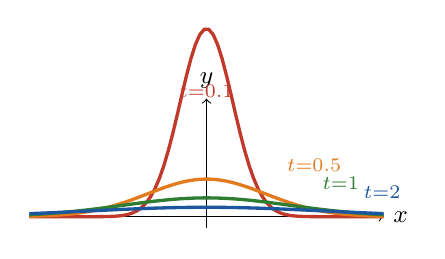
\begin{tikzpicture}[scale=0.75]
\draw[->] (-3,0) -- (3,0) node[right] {\small $x$};
\draw[->] (0,-0.2) -- (0,2) node[above] {\small $y$};
\draw[warnred, very thick, domain=-3:3, samples=80] plot (\x, {1.784/sqrt(0.1*pi)*exp(-\x*\x/(4*0.1))});
\draw[accentorange, very thick, domain=-3:3, samples=80] plot (\x, {0.798/sqrt(0.5*pi)*exp(-\x*\x/(4*0.5))});
\draw[accentgreen, very thick, domain=-3:3, samples=80] plot (\x, {0.564/sqrt(1.0*pi)*exp(-\x*\x/4)});
\draw[headerblue, very thick, domain=-3:3, samples=80] plot (\x, {0.399/sqrt(2.0*pi)*exp(-\x*\x/8)});
\node[warnred, above] at (0,1.85) {\scriptsize $t{=}0.1$};
\node[accentorange, above right] at (1.2,0.6) {\scriptsize $t{=}0.5$};
\node[accentgreen, above right] at (1.8,0.3) {\scriptsize $t{=}1$};
\node[headerblue, above right] at (2.5,0.15) {\scriptsize $t{=}2$};
\end{tikzpicture}\\[1mm]
{\footnotesize Heat kernel: spreading Gaussian as $t$ increases}
\vspace{3mm}
\begin{conceptbox}[Key Takeaway]
The Laplace transform handles nonhomogeneous boundary conditions natively --- separation of variables struggles with them. The price: the answer is a convolution integral, not a closed form.
\end{conceptbox}
\end{frame}

% ─── Slide 43: Beam Bending ───
\begin{frame}{Three-Point Beam Bending with $\delta$}
\footnotesize
\begin{examplebox}[Euler-Bernoulli Beam with Point Load]
\textbf{Equation.} Euler-Bernoulli beam with point load $F$ at $x = a$:
\[EI\,\frac{d^4 y}{dx^4} = -F\,\delta(x - a), \quad 0 < x < L\]
Simply-supported BCs: $y(0) = y(L) = 0$ and $y''(0) = y''(L) = 0$.

\medskip
\textbf{Specific case:} $L = 2$, $EI = 1$, $F = 1$, $a = 1$. So $y'''' = -\delta(x-1)$.

\textbf{Step 1.} Transform in $x$ (treat $x$ as the time-like variable):
\[s^4 Y - s^3 y(0) - s^2 y'(0) - s\, y''(0) - y'''(0) = -e^{-s}\]
Apply $y(0) = 0$ and $y''(0) = 0$. Let $C_1 = y'(0)$, $C_2 = y'''(0)$:
\[Y(s) = \frac{-e^{-s}}{s^4} + \frac{C_1}{s^2} + \frac{C_2}{s^4}\]
\end{examplebox}
\end{frame}

% ─── Slide 43 (cont.): Beam Bending --- inversion & BCs ───
\begin{frame}{Three-Point Beam Bending with $\delta$ (cont.)}
\footnotesize
\begin{examplebox}[Euler-Bernoulli Beam --- Inversion and BCs]
\textbf{Step 2.} Invert using the second shifting property (for $e^{-s}$) and table lookup:
\[y(x) = -\frac{(x-1)^3}{6}\, u(x-1) + C_1\, x + \frac{C_2\, x^3}{6}\]

\textbf{Step 3.} Apply the right-end BCs $y(2) = 0$ and $y''(2) = 0$ (here $u(x-1) = 1$):
\begin{align*}
y(2) &= -\tfrac{1}{6} + 2C_1 + \tfrac{4C_2}{3} = 0 \\
y''(2) &= -1 + 2C_2 = 0 \;\Rightarrow\; C_2 = \tfrac{1}{2}
\end{align*}
Solving: $C_1 = -\tfrac{1}{4}$.

\textbf{Answer:} $y(x) = -\frac{(x-1)^3}{6}\, u(x-1) - \frac{x}{4} + \frac{x^3}{12}$.
\end{examplebox}
\end{frame}

% ─── Slide 43 (cont.): Beam diagram & takeaway ───
\begin{frame}{Three-Point Beam Bending with $\delta$ (cont.)}
\footnotesize
\centering
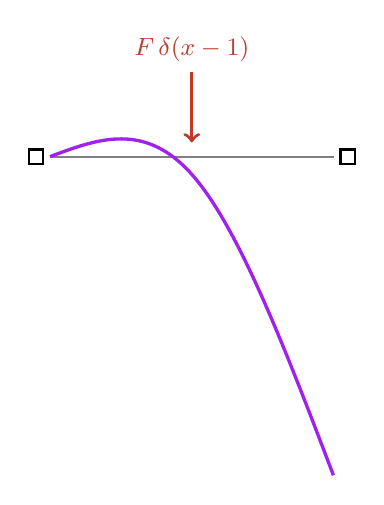
\begin{tikzpicture}[scale=0.9]
\draw[thick, gray] (0,0) -- (4,0);
\draw[thick] (-0.3,-0.1) -- (-0.3,0.1) -- (-0.1,0.1) -- (-0.1,-0.1) -- cycle;
\draw[thick] (4.1,-0.1) -- (4.1,0.1) -- (4.3,0.1) -- (4.3,-0.1) -- cycle;
\draw[->, warnred, very thick] (2,1.2) -- (2,0.2);
\node[warnred, above] at (2,1.2) {\small $F\,\delta(x-1)$};
\draw[workpurple, very thick, domain=0:4, samples=100] plot (\x, {-(-(\x-2)^3/6*(\x>2 ? 1:0) - \x/4 + \x^3/12)*1.5});
\end{tikzpicture}
\vspace{1mm}
\begin{conceptbox}[Key Takeaway]
Point loads on beams are naturally modeled by $\delta(x-a)$. The Laplace transform (in the spatial variable $x$) handles them exactly --- no need to split the beam into segments and match BCs at the load point.
\end{conceptbox}
\end{frame}

% ─── Slide 44: Abel's Tautochrone ───
\begin{frame}{Abel's Problem and the Cycloid}
\footnotesize
\begin{examplebox}[The Historical Jewel]
\textbf{Setup.} A bead slides frictionlessly down a wire from height $y$ to the origin under gravity. Abel's problem: given the descent-time function $T(y)$, find the wire's shape.

\textbf{Conservation of energy} gives $dt = -ds / \sqrt{2g(y-v)}$. Integrating from $v = y$ to $v = 0$:
\[T(y) = \frac{1}{\sqrt{2g}} \int_0^y \frac{f(v)}{\sqrt{y - v}}\, dv\]
where $f(v) = \sqrt{1 + (dx/dy)^2}$. This is a \emph{convolution}: $T = \frac{1}{\sqrt{2g}}\, (y^{-1/2} * f)$.

\textbf{Apply $\mathcal{L}$} and use $\mathcal{L}\{y^{-1/2}\} = \sqrt{\pi/s}$:
\[\mathcal{L}\{T\} = \frac{1}{\sqrt{2g}}\sqrt{\frac{\pi}{s}}\,\mathcal{L}\{f\} \;\Rightarrow\; \mathcal{L}\{f\} = \sqrt{\frac{2g}{\pi}}\, s^{-1/2}\,\mathcal{L}\{T\}\]
\end{examplebox}
\end{frame}

% ─── Slide 44 (cont.): Abel --- tautochrone solution ───
\begin{frame}{Abel's Problem and the Cycloid (cont.)}
\footnotesize
\begin{examplebox}[The Historical Jewel (cont.)]
\textbf{Tautochrone.} Set $T(y) = T_0$ (constant --- same descent time from any height). Then $\mathcal{L}\{f\} = \sqrt{2g/\pi}\, T_0\, s^{-3/2}$, which inverts to $f(y) = b/\sqrt{y}$ with $b = \sqrt{2g}\,T_0/\pi$.

\textbf{Solve} $(dx/dy)^2 = (b-y)/y$. Parametrize $y = b\sin^2\phi$ and integrate. With $a = b/2$ and $\theta = 2\phi$:
\[x = a(\theta + \sin\theta), \quad y = a(1 - \cos\theta)\]

\textbf{This is a cycloid} --- the curve traced by a point on a rolling circle. Huygens (1673) discovered the tautochrone property geometrically; Abel (1826) derived it analytically via this integral-equation approach \emph{without knowing the answer in advance}.
\end{examplebox}
\end{frame}

% ─── Slide 44 (cont.): cycloid diagram ───
\begin{frame}{Abel's Problem and the Cycloid (cont.)}
\footnotesize
\centering
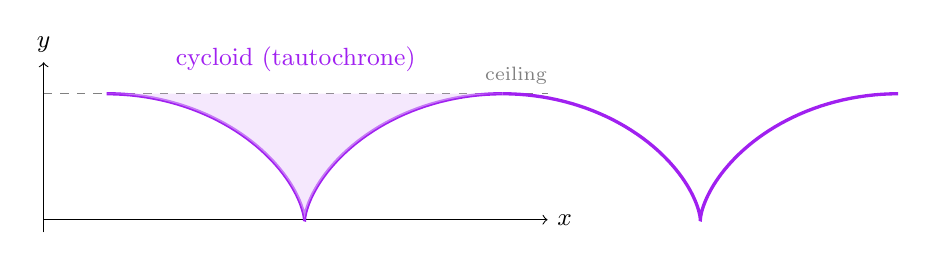
\begin{tikzpicture}[scale=0.8]
\draw[->] (0,0) -- (8,0) node[right] {\small $x$};
\draw[->] (0,-0.2) -- (0,2.5) node[above] {\small $y$};
\draw[gray, dashed] (0,2) -- (8,2);
\node[gray, above] at (7.5,2) {\scriptsize ceiling};
% Cycloid arches
\draw[workpurple, very thick, domain=0:2*pi, samples=100] plot ({1 + \x + sin(\x r)}, {2 - (1 - cos(\x r))});
\draw[workpurple, very thick, domain=2*pi:4*pi, samples=100] plot ({1 + \x + sin(\x r)}, {2 - (1 - cos(\x r))});
\fill[workpurple!20, opacity=0.5, domain=0:2*pi, samples=100] plot ({1 + \x + sin(\x r)}, {2 - (1 - cos(\x r))}) -- (1+2*pi, 2) -- (1, 2) -- cycle;
\node[workpurple, above] at (4, 2.2) {\small cycloid (tautochrone)};
\end{tikzpicture}
\vspace{1mm}
\begin{conceptbox}[Key Takeaway]
Abel's problem reduces to a convolution integral equation $T = \frac{1}{\sqrt{2g}}(y^{-1/2} * f)$, which the Laplace transform solves algebraically. The tautochrone is a cycloid --- a result Huygens found geometrically, Abel found analytically.
\end{conceptbox}
\end{frame}

% ─── Slide 45: Real-Integral Tricks ───
\begin{frame}{Evaluating Real Integrals via Laplace}
\footnotesize
\begin{columns}[T]
\begin{column}{0.42\textwidth}
\begin{formulabox}[The Trick]
From the integration-in-$s$ rule $\mathcal{L}\{f(t)/t\} = \int_s^{\infty} F(u)\, du$, take $s \to 0^+$:
\[\int_0^{\infty} \frac{f(t)}{t}\, dt = \int_0^{\infty} F(u)\, du\]
If the RHS is computable from a known transform $F = \mathcal{L}\{f\}$, a hard real integral is evaluated.
\end{formulabox}
\end{column}
\begin{column}{0.56\textwidth}
\begin{examplebox}[Dirichlet Integral]
Use $\mathcal{L}\{\sin t\} = \frac{1}{s^2+1}$. Then
\resizeeq{\int_0^{\infty} \frac{\sin t}{t}\, dt = \int_0^{\infty} \frac{1}{u^2+1}\, du = \arctan(u)\Big|_0^{\infty} = \frac{\pi}{2}}
The famous Dirichlet integral in two lines.
\end{examplebox}
\vspace{0.5mm}
\begin{examplebox}[Frullani-Type Integral]
Use $\mathcal{L}\{e^{-at}\} = \frac{1}{s+a}$. Then
\resizeeq{\int_0^{\infty} \frac{e^{-at} - e^{-bt}}{t}\, dt = \int_0^{\infty}\!\left[\frac{1}{u+a} - \frac{1}{u+b}\right]du = \ln\frac{b}{a}}
\end{examplebox}
\vspace{0.5mm}
\begin{examplebox}[Damped Sine Integral]
Use $\mathcal{L}\{e^{-at}\sin(bt)\} = \frac{b}{(s+a)^2+b^2}$. Then
\[\int_0^{\infty} \frac{e^{-at}\sin(bt)}{t}\, dt = \arctan\frac{b}{a}\]
\end{examplebox}
\end{column}
\end{columns}
\end{frame}

% ─── Slide 45 (cont.): Real Integrals takeaway ───
\begin{frame}{Evaluating Real Integrals via Laplace (cont.)}
\footnotesize
\begin{conceptbox}[Key Takeaway]
The Laplace transform is not just for ODEs --- it is a general integration tool. Any time a $1/t$ factor appears in a real integral, consider $\mathcal{L}\{f(t)/t\} = \int_s^{\infty} F$.
\end{conceptbox}
\end{frame}

% ─── Slide 46: Resonance via Convolution ───
\begin{frame}{Resonance Emerges Naturally from Convolution}
\footnotesize
\begin{columns}[T]
\begin{column}{0.58\textwidth}
\begin{examplebox}[Driving at the Natural Frequency]
Consider $x'' + \omega_0^2 x = \cos(\omega_0 t)$, $x(0) = x'(0) = 0$ --- drive at the natural frequency.

From Duhamel's principle:
\[x(t) = \int_0^t \frac{\sin(\omega_0(t-\tau))}{\omega_0}\, \cos(\omega_0 \tau)\, d\tau\]

Use the product-to-sum identity $\sin A \cos B = \tfrac{1}{2}[\sin(A+B) + \sin(A-B)]$:
\resizeeq{\sin(\omega_0(t-\tau))\cos(\omega_0\tau) = \tfrac{1}{2}[\sin(\omega_0 t) + \sin(\omega_0(t-2\tau))]}

Integrate:
\begin{align*}
x(t) &= \frac{1}{2\omega_0}\int_0^t [\sin(\omega_0 t) + \sin(\omega_0(t-2\tau))]\, d\tau \\
&= \frac{1}{2\omega_0}\!\left[t\sin(\omega_0 t) + \frac{\cos(\omega_0(t-2\tau))}{2\omega_0}\Big|_0^t\right] \\
&= \frac{t\,\sin(\omega_0 t)}{2\omega_0}
\end{align*}
(The cosine terms cancel since $\cos(-\theta) = \cos\theta$.)

\textbf{Result:} $x(t) = \frac{t\,\sin(\omega_0 t)}{2\omega_0}$ --- amplitude grows linearly with $t$.
\end{examplebox}
\end{column}
\begin{column}{0.38\textwidth}
\centering
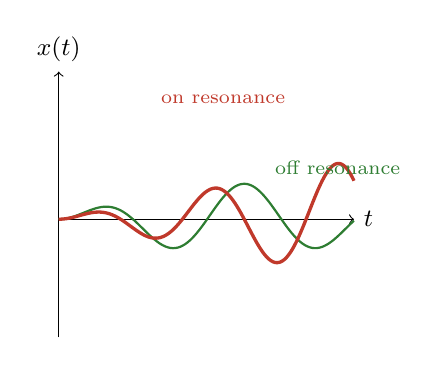
\begin{tikzpicture}[scale=0.75]
\draw[->] (0,0) -- (5,0) node[right] {\small $t$};
\draw[->] (0,-2) -- (0,2.5) node[above] {\small $x(t)$};
\draw[accentgreen, thick, domain=0:5, samples=120] plot (\x, {0.3*cos(2*\x r) - 0.3*cos(3*\x r)});
\draw[warnred, very thick, domain=0:5, samples=150] plot (\x, {0.2*\x*sin(3*\x r)});
\node[accentgreen, above right] at (3.5,0.6) {\scriptsize off resonance};
\node[warnred, above left] at (4,1.8) {\scriptsize on resonance};
\end{tikzpicture}
\vspace{1mm}
\begin{conceptbox}[Key Takeaway]
Resonance is not a special case to be memorized. It falls out of the convolution integral naturally when the forcing frequency matches a natural frequency --- the $t$ factor in front of the sine is the signature.
\end{conceptbox}
\end{column}
\end{columns}
\end{frame}

% ═══════════════════════════════════════════════════════════════════
% PART VI --- REFERENCE & CLOSING
% ═══════════════════════════════════════════════════════════════════

\section{Part VI --- Reference \& Closing}

% ─── Slide 47: Section Header Part VI ───
{
\setbeamercolor{background canvas}{bg=headerblue}
\setbeamertemplate{footline}{}
\begin{frame}[plain]
\vspace{2cm}
{\color{accentorange}\Huge\textbf{PART VI}}\\[0.4cm]
{\color{white}\Huge\textbf{Reference Tables \& Examples}}\\[0.8cm]
{\color{white!85}\large Master Laplace and inverse-Laplace tables. Encyclopedic worked examples.\\
Historical sketches. Cheat-sheet summary. Closing.}
\end{frame}
}

% ─── Slide 48: Master Laplace Transform Table ───
\begin{frame}{Master Table of Laplace Transforms}
\scriptsize
\centering
\begin{tabular}{@{}lll@{\hspace{4mm}}lll@{}}
\toprule
\textbf{$f(t)$} & \textbf{$F(s)$} & \textbf{Valid} & \textbf{$f(t)$} & \textbf{$F(s)$} & \textbf{Valid} \\
\midrule
$1$ & $\frac{1}{s}$ & $s>0$ & $u_a(t)$ & $\frac{e^{-as}}{s}$ & $s>0$ \\
$t$ & $\frac{1}{s^2}$ & $s>0$ & $u_a(t)f(t\!-\!a)$ & $e^{-as}F(s)$ & $s>\alpha$ \\
$t^n$ & $\frac{n!}{s^{n+1}}$ & $s>0$ & $e^{at}f(t)$ & $F(s\!-\!a)$ & $s>\alpha{+}a$ \\
$t^\alpha$ & $\frac{\Gamma(\alpha{+}1)}{s^{\alpha+1}}$ & $s>0$ & $f(ct)$ & $\frac{1}{c}F(s/c)$ & $c>0$ \\
$e^{at}$ & $\frac{1}{s-a}$ & $s>a$ & $\delta(t\!-\!t_0)$ & $e^{-st_0}$ & all $s$ \\
$\sin(at)$ & $\frac{a}{s^2+a^2}$ & $s>0$ & $f'(t)$ & $sF - f(0)$ & $s>\alpha$ \\
$\cos(at)$ & $\frac{s}{s^2+a^2}$ & $s>0$ & $f''(t)$ & $s^2F - sf(0) - f'(0)$ & $s>\alpha$ \\
$\sinh(at)$ & $\frac{a}{s^2-a^2}$ & $s>|a|$ & $f^{(n)}(t)$ & $s^nF - \sum s^{n-1-k}f^{(k)}(0)$ & $s>\alpha$ \\
$\cosh(at)$ & $\frac{s}{s^2-a^2}$ & $s>|a|$ & $\int_0^t f\,d\tau$ & $\frac{F(s)}{s}$ & $s>\alpha$ \\
$e^{at}\sin(bt)$ & $\frac{b}{(s-a)^2+b^2}$ & $s>a$ & $(f*g)(t)$ & $F(s)\,G(s)$ & $s>\max(\alpha,\beta)$ \\
$e^{at}\cos(bt)$ & $\frac{s-a}{(s-a)^2+b^2}$ & $s>a$ & $t\sin(at)$ & $\frac{2as}{(s^2+a^2)^2}$ & $s>0$ \\
$t^n e^{at}$ & $\frac{n!}{(s-a)^{n+1}}$ & $s>a$ & $t\cos(at)$ & $\frac{s^2-a^2}{(s^2+a^2)^2}$ & $s>0$ \\
\bottomrule
\end{tabular}
\vspace{1mm}
\begin{conceptbox}[Usage]
Recognize the $s$-domain pattern, then apply the corresponding rule. Shifting for $(s-a)$ patterns; second shifting for $e^{-as}$ factors; convolution for products $F(s)G(s)$.
\end{conceptbox}
\end{frame}

% ─── Slide 49: Master Inverse Laplace Table ───
\begin{frame}{Master Table of Inverse Laplace Transforms}
\scriptsize
\centering
\begin{tabular}{@{}lll@{\hspace{4mm}}lll@{}}
\toprule
\textbf{$F(s)$ pattern} & \textbf{$f(t)$} & \textbf{Technique} & \textbf{$F(s)$ pattern} & \textbf{$f(t)$} & \textbf{Technique} \\
\midrule
$\frac{1}{s}$ & $1$ & Direct & $\frac{e^{-as}}{s}$ & $u_a(t)$ & 2nd shift \\
$\frac{1}{s^n}$ & $\frac{t^{n-1}}{(n-1)!}$ & Direct & $\frac{e^{-as}}{s-a}$ & $u_a(t)\,e^{a(t-a)}$ & 2nd shift \\
$\frac{1}{s-a}$ & $e^{at}$ & Direct & $\frac{b\,e^{-as}}{(s-a)^2+b^2}$ & $u_a\,e^{a(t-a)}\!\sin b(t\!-\!a)$ & 2nd shift \\
$\frac{a}{s^2+a^2}$ & $\sin(at)$ & Direct & $e^{-as}F(s)$ & $u_a(t)\,f(t-a)$ & 2nd shift (gen.) \\
$\frac{s}{s^2+a^2}$ & $\cos(at)$ & Direct & $\frac{F(s)}{s}$ & $\int_0^t f\,d\tau$ & Integration \\
$\frac{a}{s^2-a^2}$ & $\sinh(at)$ & Direct & $F(s)\,G(s)$ & $(f*g)(t)$ & Convolution \\
$\frac{s}{s^2-a^2}$ & $\cosh(at)$ & Direct & $1$ & $\delta(t)$ & Delta \\
$\frac{n!}{(s-a)^{n+1}}$ & $t^n e^{at}$ & Direct & $e^{-as}$ & $\delta(t-a)$ & Delta \\
$\frac{b}{(s-a)^2+b^2}$ & $e^{at}\sin(bt)$ & 1st shift & $-F'(s)$ & $t\,f(t)$ & Diff. in $s$ \\
$\frac{s-a}{(s-a)^2+b^2}$ & $e^{at}\cos(bt)$ & 1st shift & $\int_s^\infty F\,du$ & $\frac{f(t)}{t}$ & Integ. in $s$ \\
$\frac{1}{(s-a)(s-b)}$ & $\frac{e^{at}-e^{bt}}{a-b}$ & Partial frac. & $\frac{1}{\sqrt{s^2+a^2}}$ & $J_0(at)$ & Bessel \\
$\frac{1}{(s-a)^2}$ & $t\,e^{at}$ & Partial frac. & $\frac{As+B}{(s-a)^2+b^2}$ & $e^{at}[C_1\sin bt + C_2\cos bt]$ & Comp. square \\
\bottomrule
\end{tabular}
\vspace{1mm}
\begin{conceptbox}[Usage]
Inverse-Laplace lookup works by pattern matching. See $(s-a)^2+b^2$ $\to$ first shifting; see $e^{-as}$ $\to$ second shifting; see $F(s)G(s)$ $\to$ convolution.
\end{conceptbox}
\end{frame}

% ─── Slide 50: Purple Worked Examples — Forward Transforms ───
\begin{frame}{Worked Examples --- Forward Transforms}
\footnotesize
\begin{columns}[T]
\begin{column}{0.48\textwidth}
\begin{examplebox}[Polynomial $\times$ Exponential]
\textbf{Problem.} Find $\mathcal{L}\{t^2 e^{-3t}\}$.

Use $\mathcal{L}\{t^n e^{at}\} = \frac{n!}{(s-a)^{n+1}}$ with $n = 2, a = -3$:
\resizeeq{\mathcal{L}\{t^2 e^{-3t}\} = \frac{2!}{(s+3)^3} = \frac{2}{(s+3)^3}, \quad s > -3}
\end{examplebox}
\vspace{0.5mm}
\begin{examplebox}[Trig via Euler]
\textbf{Problem.} Find $\mathcal{L}\{\sin(3t)\cos(5t)\}$.

Use $\sin A \cos B = \tfrac{1}{2}[\sin(A+B) + \sin(A-B)]$:
\[\sin(3t)\cos(5t) = \tfrac{1}{2}[\sin(8t) - \sin(2t)]\]
\[\mathcal{L}\{\cdots\} = \frac{1}{2}\!\left[\frac{8}{s^2+64} - \frac{2}{s^2+4}\right]\]
\end{examplebox}
\end{column}
\begin{column}{0.48\textwidth}
\begin{examplebox}[Hyperbolic via Linearity]
\textbf{Problem.} Find $\mathcal{L}\{\cosh(at)\}$.

Use $\cosh(at) = \frac{e^{at}+e^{-at}}{2}$:
\resizeeq{\mathcal{L}\{\cosh(at)\} = \tfrac{1}{2}\!\left[\frac{1}{s-a} + \frac{1}{s+a}\right] = \frac{s}{s^2-a^2}}
for $s > |a|$.
\end{examplebox}
\vspace{0.5mm}
\begin{examplebox}[Piecewise Function]
\textbf{Problem.} Find $\mathcal{L}\{f\}$ where $f(t) = 0$ for $t<1$, $t-1$ for $1<t<3$, $2$ for $t>3$.

Write $f(t) = (t-1)u_1(t) - (t-3)u_3(t)$. By the second shifting property:
\[\mathcal{L}\{f\} = \frac{e^{-s}}{s^2} - \frac{e^{-3s}}{s^2} = \frac{e^{-s}-e^{-3s}}{s^2}\]
\end{examplebox}
\end{column}
\end{columns}
\end{frame}

% ─── Slide 51: Purple Worked Examples — Inverse Transforms ───
\begin{frame}{Worked Examples --- Inverse Transforms}
\footnotesize
\begin{columns}[T]
\begin{column}{0.48\textwidth}
\begin{examplebox}[Distinct Linear Factors]
\textbf{Problem.} $\mathcal{L}^{-1}\!\left\{\frac{3s-14}{(s-5)(s-2)}\right\}$

Partial fractions: $\frac{A}{s-5} + \frac{B}{s-2}$. Solve: $A = \tfrac{1}{3}, B = \tfrac{8}{3}$.
\[\mathcal{L}^{-1}\{\cdots\} = \tfrac{1}{3}e^{5t} + \tfrac{8}{3}e^{2t}\]
\end{examplebox}
\end{column}
\begin{column}{0.48\textwidth}
\begin{examplebox}[Delayed (Heaviside)]
\textbf{Problem.} $\mathcal{L}^{-1}\!\left\{\frac{e^{-4s}}{s^2+9}\right\}$

Without $e^{-4s}$: $\mathcal{L}^{-1}\!\left\{\frac{1}{s^2+9}\right\} = \tfrac{1}{3}\sin(3t)$. With $e^{-4s}$, apply second shifting:
\[\mathcal{L}^{-1}\{\cdots\} = u_4(t)\cdot\tfrac{1}{3}\sin(3(t-4))\]
A sine wave switching on at $t = 4$.
\end{examplebox}
\end{column}
\end{columns}
\end{frame}

% ─── Slide 51 (cont.): inverse-transform examples 3 & 4 ───
\begin{frame}{Worked Examples --- Inverse Transforms (cont.)}
\footnotesize
\begin{columns}[T]
\begin{column}{0.48\textwidth}
\begin{examplebox}[Irreducible Quadratic]
\textbf{Problem.} $\mathcal{L}^{-1}\!\left\{\frac{2s+3}{s^2+2s+5}\right\}$

Complete the square: $s^2+2s+5 = (s+1)^2+4$. Rewrite numerator: $2s+3 = 2(s+1)+1$.
\[\frac{2(s+1)}{(s+1)^2+2^2} + \frac{1}{2}\cdot\frac{2}{(s+1)^2+2^2}\]
Apply first shifting:
\[\mathcal{L}^{-1}\{\cdots\} = 2e^{-t}\cos(2t) + \tfrac{1}{2}e^{-t}\sin(2t)\]
\end{examplebox}
\end{column}
\begin{column}{0.48\textwidth}
\begin{examplebox}[Convolution]
\textbf{Problem.} $\mathcal{L}^{-1}\!\left\{\frac{1}{s^2(s+1)}\right\}$

Write as product: $\frac{1}{s^2}\cdot\frac{1}{s+1}$. Inverses: $t$ and $e^{-t}$. Convolve:
\resizeeq{\mathcal{L}^{-1}\{\cdots\} = (t) * (e^{-t}) = \int_0^t (t-\tau)\,e^{-\tau}\,d\tau = t + e^{-t} - 1}
\end{examplebox}
\end{column}
\end{columns}
\end{frame}

% ─── Slide 52: Purple Worked Examples — Solving IVPs ───
\begin{frame}{Worked Examples --- Solving IVPs}
\footnotesize
\begin{columns}[T]
\begin{column}{0.48\textwidth}
\begin{examplebox}[Simple Homogeneous]
\textbf{Problem.} $y'' - 4y' + 4y = 0$, $y(0)=1, y'(0)=0$.

Transform: $(s-2)^2 Y = s$. Rewrite: $s = (s-2)+2$.
\[Y = \frac{1}{s-2} + \frac{2}{(s-2)^2}\]
\textbf{Answer:} $y(t) = (1+2t)\,e^{2t}$.
\end{examplebox}
\end{column}
\begin{column}{0.48\textwidth}
\begin{examplebox}[Step Forcing]
\textbf{Problem.} $y' + y = u_3(t)$, $y(0)=1$.

Transform: $(s+1)Y = 1 + \frac{e^{-3s}}{s}$.
\resizeeq{Y = \frac{1}{s+1} + \frac{e^{-3s}}{s(s+1)} = \frac{1}{s+1} + e^{-3s}\!\left(\frac{1}{s} - \frac{1}{s+1}\right)}
\textbf{Answer:} $y(t) = e^{-t} + u_3(t)[1 - e^{-(t-3)}]$.
\end{examplebox}
\end{column}
\end{columns}
\end{frame}

% ─── Slide 52 (cont.): IVP examples --- forced & impulse ───
\begin{frame}{Worked Examples --- Solving IVPs (cont.)}
\footnotesize
\begin{columns}[T]
\begin{column}{0.48\textwidth}
\begin{examplebox}[Forced Oscillation]
\textbf{Problem.} $y'' + 9y = \sin(2t)$, $y(0)=y'(0)=0$.

Transform: $(s^2+9)Y = \frac{2}{s^2+4}$.
\[Y = \frac{2}{(s^2+4)(s^2+9)} = \frac{2/5}{s^2+4} - \frac{2/5}{s^2+9}\]
\textbf{Answer:} $y(t) = \tfrac{1}{5}\sin(2t) - \tfrac{2}{15}\sin(3t)$.
\end{examplebox}
\end{column}
\begin{column}{0.48\textwidth}
\begin{examplebox}[Impulse Forcing]
\textbf{Problem.} $y'' + 4y = \delta(t-\pi)$, $y(0)=1, y'(0)=0$.

Transform: $Y = \frac{s}{s^2+4} + \frac{e^{-\pi s}}{s^2+4}$.

Invert: $\cos(2t)$ for the first term; second shifting for $e^{-\pi s}$:
\[y(t) = \cos(2t) + u_\pi(t)\cdot\tfrac{1}{2}\sin(2(t-\pi))\]
Since $\sin(2(t-\pi)) = \sin(2t)$, the impulse adds a sine component at $t = \pi$.
\end{examplebox}
\end{column}
\end{columns}
\end{frame}

% ─── Slide 53: Historical Sketches ───
\begin{frame}{The People Behind the Transform}
\footnotesize
\begin{columns}[T]
\begin{column}{0.48\textwidth}
\begin{topicsbox}[Pierre-Simon Laplace (1749--1827)]
French mathematician and astronomer. His \emph{M\'ecanique C\'eleste} (5 vols, 1799--1825) developed potential theory and showed the solar system is dynamically stable. When Napoleon reportedly remarked on the absence of God in his celestial mechanics, Laplace is said to have replied that he had no need of that hypothesis. The Laplace transform appears in his \emph{Th\'eorie Analytique des Probabilit\'es} (1812).
\end{topicsbox}
\end{column}
\begin{column}{0.48\textwidth}
\begin{topicsbox}[Paul Adrien Maurice Dirac (1902--1984)]
English theoretical physicist, Nobel Prize 1933 (age 31) for the Dirac equation predicting antimatter. Introduced the delta function in \emph{The Principles of Quantum Mechanics} (1930) as a notational convenience --- its rigorous foundation as a distribution came later (Schwartz, 1940s, Fields Medal). The delta function is now indispensable in signal processing, PDEs, and quantum field theory.
\end{topicsbox}
\end{column}
\end{columns}
\end{frame}

% ─── Slide 53 (cont.): more historical sketches ───
\begin{frame}{The People Behind the Transform (cont.)}
\footnotesize
\begin{columns}[T]
\begin{column}{0.48\textwidth}
\begin{topicsbox}[Oliver Heaviside (1850--1925)]
English self-taught electrical engineer, mathematician, and physicist. Reduced Maxwell's 20 original equations to the 4 now taught. Developed operational calculus --- the forerunner of Laplace-transform methods --- to solve transmission-line problems. The unit step function bears his name. The etymology is coincidental to the function's being nonzero on one side of the origin.
\end{topicsbox}
\end{column}
\begin{column}{0.48\textwidth}
\begin{topicsbox}[Niels Henrik Abel (1802--1829)]
Norwegian mathematician, dead of tuberculosis at 26. Solved the tautochrone problem at age 18 by what is now called the Laplace-transform method. Proved the general quintic equation has no solution in radicals. Abel's theorem on integrals (1826) --- Jacobi reportedly regarded it as the greatest discovery in integral calculus of the nineteenth century. Crelle offered him a Berlin professorship; the letter arrived two days after his death.
\end{topicsbox}
\end{column}
\end{columns}
\end{frame}

% ─── Slide 54: Cheat-Sheet Summary ───
\begin{frame}{One-Page Summary --- All the Rules}
\scriptsize
\begin{columns}[T]
\begin{column}{0.32\textwidth}
\begin{formulabox}[Definition]
\[F(s) = \int_0^{\infty}\! e^{-st} f(t)\, dt\]
Exists if $f$ is piecewise continuous + exponential order.
\end{formulabox}
\vspace{0.5mm}
\begin{formulabox}[Linearity]
\[\mathcal{L}\{\alpha f + \beta g\} = \alpha F + \beta G\]
\end{formulabox}
\end{column}
\begin{column}{0.32\textwidth}
\begin{formulabox}[Shifting Properties]
\[\mathcal{L}\{e^{at}f(t)\} = F(s\!-\!a)\]
\[\mathcal{L}\{u_a(t)f(t\!-\!a)\} = e^{-as}F(s)\]
\end{formulabox}
\vspace{0.5mm}
\begin{formulabox}[Derivative Rules]
\resizeeq{\begin{aligned}
\mathcal{L}\{f'\} &= sF - f(0) \\
\mathcal{L}\{f''\} &= s^2F - sf(0) - f'(0) \\
\mathcal{L}\{f^{(n)}\} &= s^n F - \textstyle\sum_{k=0}^{n-1} s^{n-1-k} f^{(k)}(0)
\end{aligned}}
\end{formulabox}
\end{column}
\begin{column}{0.32\textwidth}
\begin{formulabox}[Special Functions]
\[\mathcal{L}\{u_a(t)\} = \frac{e^{-as}}{s}\]
\[\mathcal{L}\{\delta(t-a)\} = e^{-as}\]
\[\mathcal{L}\{\sin(at)\} = \frac{a}{s^2+a^2}\]
\[\mathcal{L}\{\cos(at)\} = \frac{s}{s^2+a^2}\]
\end{formulabox}
\end{column}
\end{columns}
\end{frame}

% ─── Slide 54 (cont.): Cheat-sheet method summary ───
\begin{frame}{One-Page Summary --- All the Rules (cont.)}
\footnotesize
\begin{formulabox}[Convolution \& Transfer]
\[(f*g)(t) = \int_0^t\! f(\tau)g(t\!-\!\tau)\, d\tau\]
\[\mathcal{L}\{f*g\} = F(s)\,G(s)\]
\[H(s) = \frac{X(s)}{F(s)} = \frac{N(s)}{P(s)}\]
\[h(t) = \mathcal{L}^{-1}\{H(s)\}\]
Poles in left half-plane $\Rightarrow$ stable.
\end{formulabox}
\vspace{0.5mm}
\begin{conceptbox}[The Method]
Transform $\to$ substitute ICs $\to$ solve algebraically $\to$ decompose ($F(s)G(s) \to$ convolution; $(s-a)^2+b^2 \to$ shifting; $(s-r)^k \to$ partial fractions) $\to$ invert.
\end{conceptbox}
\end{frame}

% ─── Slide 55: Closing ───
{
\setbeamercolor{background canvas}{bg=accentorange}
\setbeamertemplate{footline}{}
\begin{frame}[plain]
\vspace{1.2cm}
\begin{center}
{\color{white}\Huge\textbf{Three Big Ideas}}\\[0.8cm]
\begin{minipage}{0.85\textwidth}
{\color{white}\large\itshape
First: differentiation in $t$ becomes multiplication by $s$ --- the entire Laplace method follows from this single substitution.

\medskip
Second: the convolution theorem is the product rule Laplace transforms always wanted --- and it gives Duhamel's principle, transfer functions, and the impulse-response framework for free.

\medskip
Third: poles in the left half-plane mean stability --- and this single geometric picture underpins all of classical control theory.}
\end{minipage}\\[1cm]
{\color{white!85}\footnotesize\textsc{Laplace Transforms \quad\textbar\quad A Self-Study Reference Deck \quad\textbar\quad End}}
\end{center}
\end{frame}
}

\end{document}
